%% slides.tex — Apresentação TCC para banca
%% Gustavo Spellmeier Neves — INF/UFRGS
%%
%% Compile: pdflatex slides && pdflatex slides

\documentclass{beamer}

\usepackage[T1]{fontenc}
\usepackage[brazil]{babel}
\usepackage[utf8]{inputenc}
\usepackage{graphicx}
\usepackage{booktabs}
\usepackage{amsmath}
\usepackage{multirow}
\usepackage{subcaption}
\usepackage{tikz}
\usetikzlibrary{shapes.geometric, arrows.meta, positioning, calc}

% Caminho das imagens do TCC
\graphicspath{{../tcc-latex/imagens/}{../tcc-latex/imagens/analiseMapas/}}

% Tema INF
\usetheme{Inf}

% Metadados
\title[Mapas Esquemáticos via MIP]
      {Otimização Inteira Mista Aplicada à Geração de Mapas Esquemáticos de Redes de Transporte}

\subtitle{Um Estudo de Caso sobre o Sistema de Ônibus de Porto Alegre}

\date{Outubro de 2026}

\author{Gustavo Spellmeier Neves}
\institute{Instituto de Informática --- UFRGS \\ Orientador: Prof.~Dr.~Lucas Melo Schnorr}

\begin{document}

% ============================================================
% Slide de Título
% ============================================================
\InfTitlePage

% ============================================================
% Agenda
% ============================================================
% \begin{frame}
%   \frametitle{Agenda}
%   \tableofcontents
% \end{frame}

% ============================================================
\section{Introdução e Motivação}
% ============================================================

\begin{frame}[plain]
  \sectionpage
\end{frame}

\begin{frame}{Contexto}
  \begin{itemize}
    \item Redes de transporte público são parte essencial do cotidiano urbano
    \item Porto Alegre: ${\sim}300$ linhas de ônibus, ${\sim}4.000$ paradas
    \item Ferramentas como Moovit planejam rotas individuais, mas \textbf{não oferecem uma visão geral e esquematizada} da rede
    \item Ausência de mapas consultáveis \textbf{offline}, sem necessidade de internet ou dispositivos eletrônicos
  \end{itemize}
\end{frame}

\begin{frame}{Mapas Esquemáticos: Por Quê?}
  \begin{columns}[c]
    \begin{column}{0.48\textwidth}
      \centering
      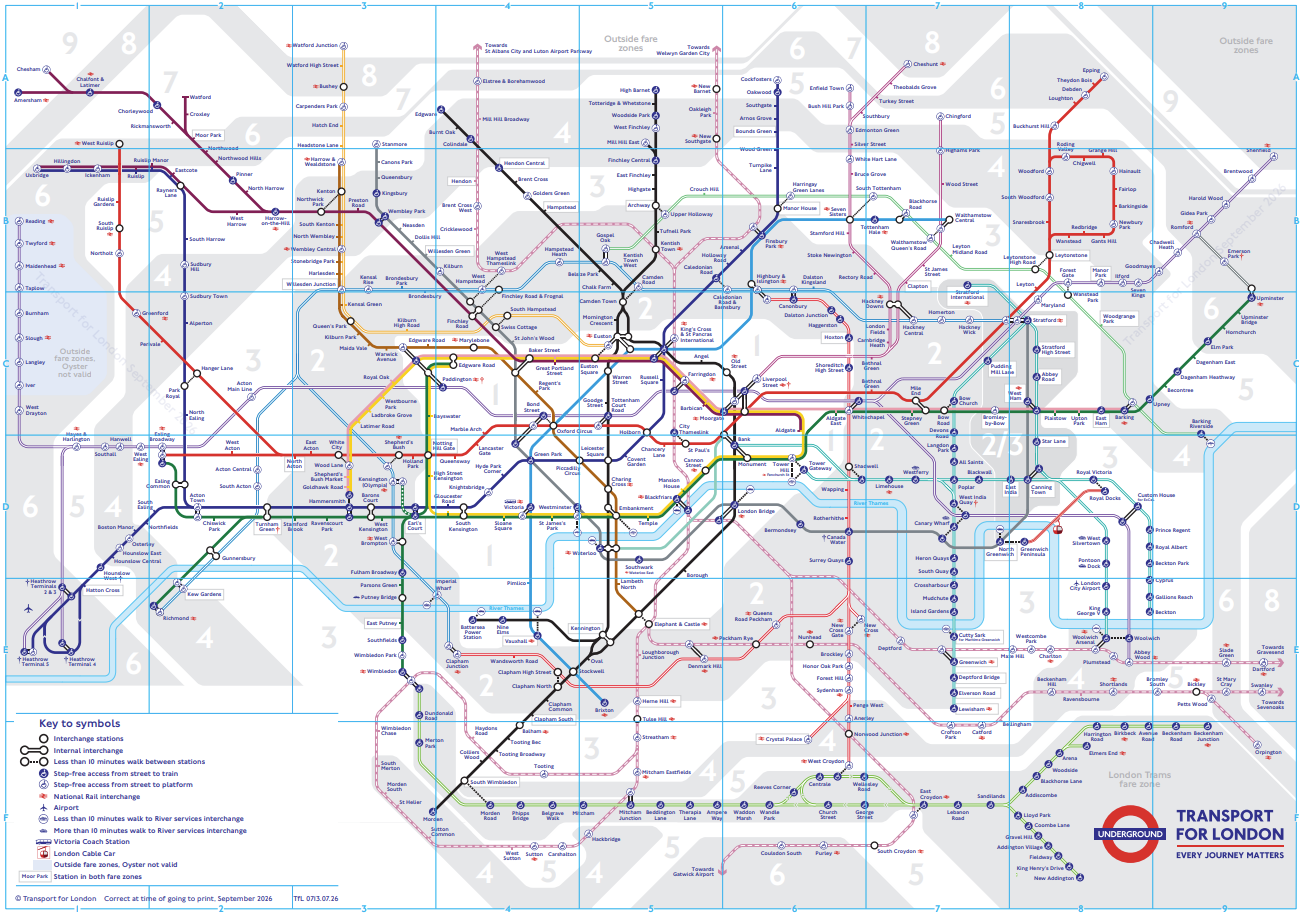
\includegraphics[width=\linewidth]{mapa_esquematico_londres.png}\\
      {\scriptsize Metrô de Londres (Harry Beck, 1933)}
    \end{column}
    \begin{column}{0.48\textwidth}
      \centering
      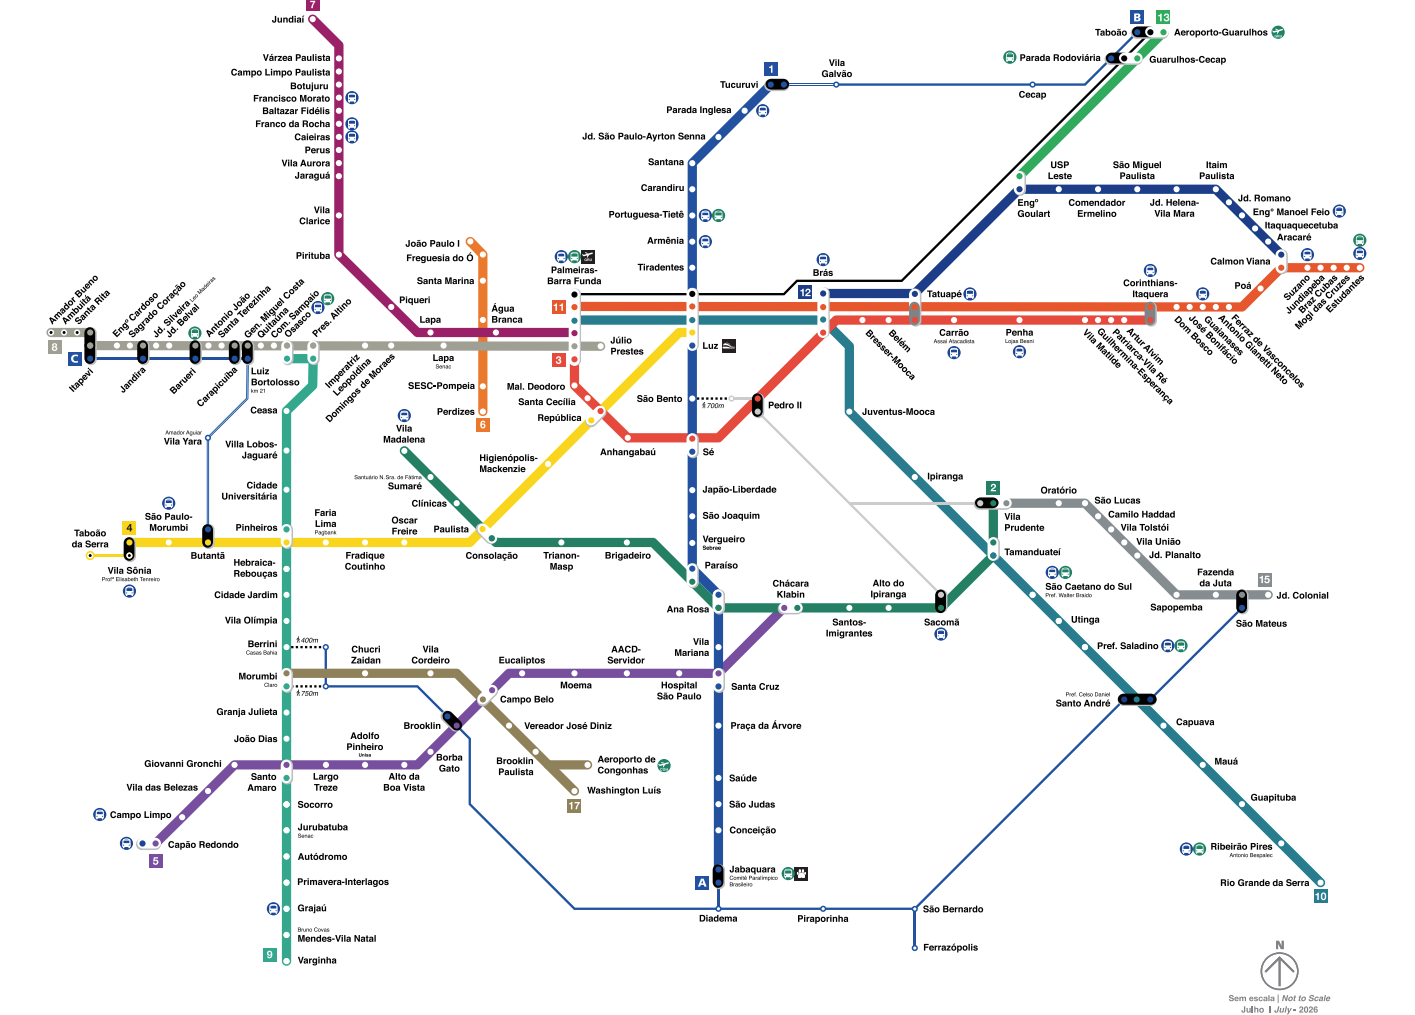
\includegraphics[width=\linewidth]{mapa_esquematico_saopaulo.png}\\
      {\scriptsize Rede Metropolitana de São Paulo}
    \end{column}
  \end{columns}
  \vspace{0.3cm}
  \begin{itemize}
    \item Abstraem a geografia para priorizar \textbf{legibilidade}
    \item Princípios: octilinearidade, minimização de curvas, preservação topológica
    \item Elaboração manual é cara e lenta — motivação para \textbf{automação} (Modelo de Nöllenburg e Wolff)
  \end{itemize}
\end{frame}

\begin{frame}{Desafios em Porto Alegre}
  \begin{itemize}
    \item \textbf{Inexistência de um grafo formal} da rede de ônibus
      \begin{itemize}
        \item Dados GTFS da EPTC: itinerários operacionais e coordenadas brutas
        \item Sem topologia unificada conectada
      \end{itemize}
    \item \textbf{Escala e complexidade computacional}
      \begin{itemize}
        \item Redes de metrô clássicas: dezenas a centenas de estações
        \item Porto Alegre: 3.831 paradas, 4.382 arestas
      \end{itemize}
    \item Aplicação direta do modelo clássico (Nöllenburg e Wolff) \textbf{não convergiu} em testes preliminares
  \end{itemize}
\end{frame}

\begin{frame}{Objetivo}
  \textbf{Objetivo:} Investigar a viabilidade de modelar, simplificar e esquematizar automaticamente a malha de ônibus de Porto Alegre via otimização linear.

  \vspace{0.3cm}
  \textbf{Etapas:}
  \begin{enumerate}
    \item Construção do grafo base a partir de dados da EPTC
    \item Pipeline de abstração e simplificação topológica
    \item Adaptação de formulações MIP
    \item Validação empírica sobre a malha das bacias operacionais de Porto Alegre
  \end{enumerate}
\end{frame}

% % ============================================================
% \section{Trabalhos Relacionados}
% % ============================================================

% \begin{frame}{Trabalhos Relacionados}
%   \begin{itemize}
%     \item \textbf{Nöllenburg e Wolff (2011):} Modelo MIP seminal para redes de metrô (Sydney, Londres)
%     \item \textbf{Oke e Siddiqui (2015):} Simplificações computacionais — relaxação de coordenadas, modelo biobjetivo
%     \item \textbf{Sadahiro et al. (2016):} Foco em mapas de ônibus, mas preserva escala geográfica 1:1
%     \item \textbf{Brosi e Bast (2023):} Escala global via OpenStreetMap, mas exclui ônibus por complexidade
%   \end{itemize}
%   \vspace{0.3cm}
%   \textbf{Lacuna:} Nenhum trabalho aplica otimização exata (MIP) a uma rede de ônibus urbana de larga escala a partir de dados abertos GTFS.
% \end{frame}

% \begin{frame}{Comparativo: Sydney}
%   \begin{columns}[c]
%     \begin{column}{0.48\textwidth}
%       \centering
%       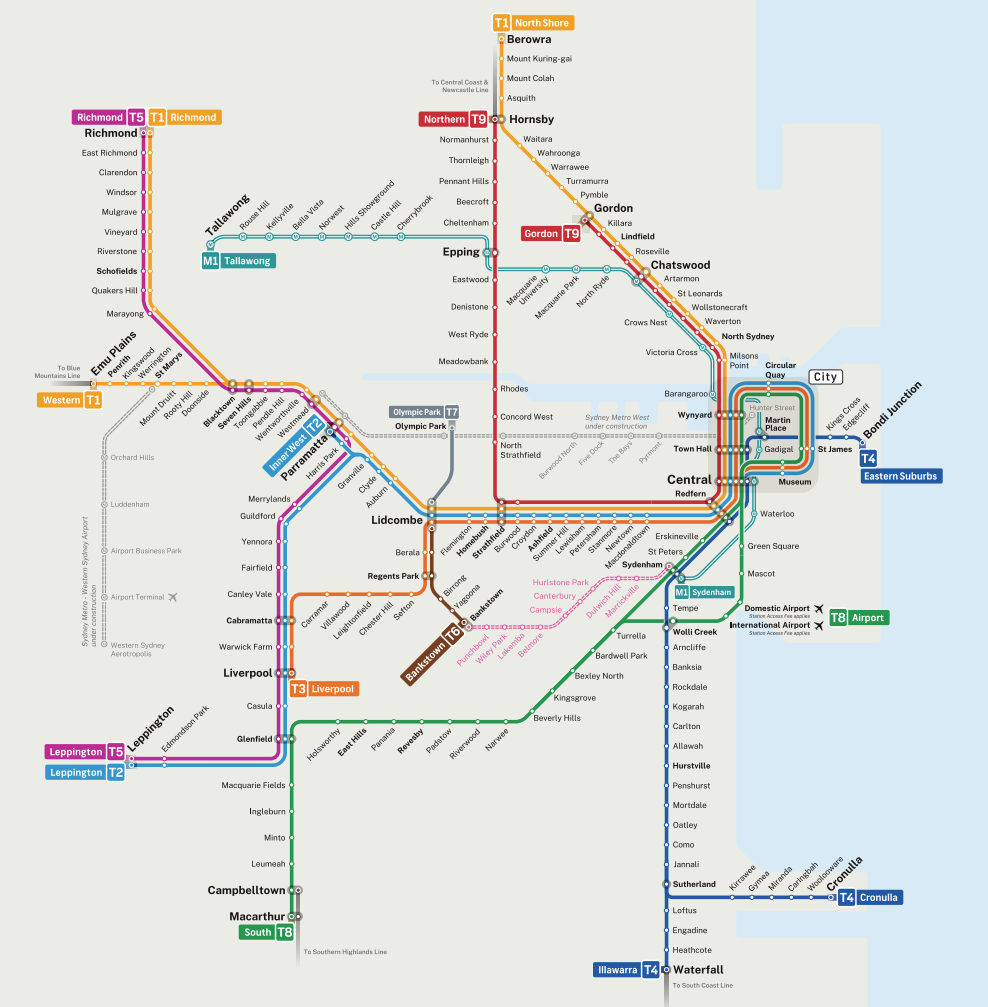
\includegraphics[width=\linewidth]{sydney_original.png}\\
%       {\scriptsize Mapa oficial de Sydney}
%     \end{column}
%     \begin{column}{0.48\textwidth}
%       \centering
%       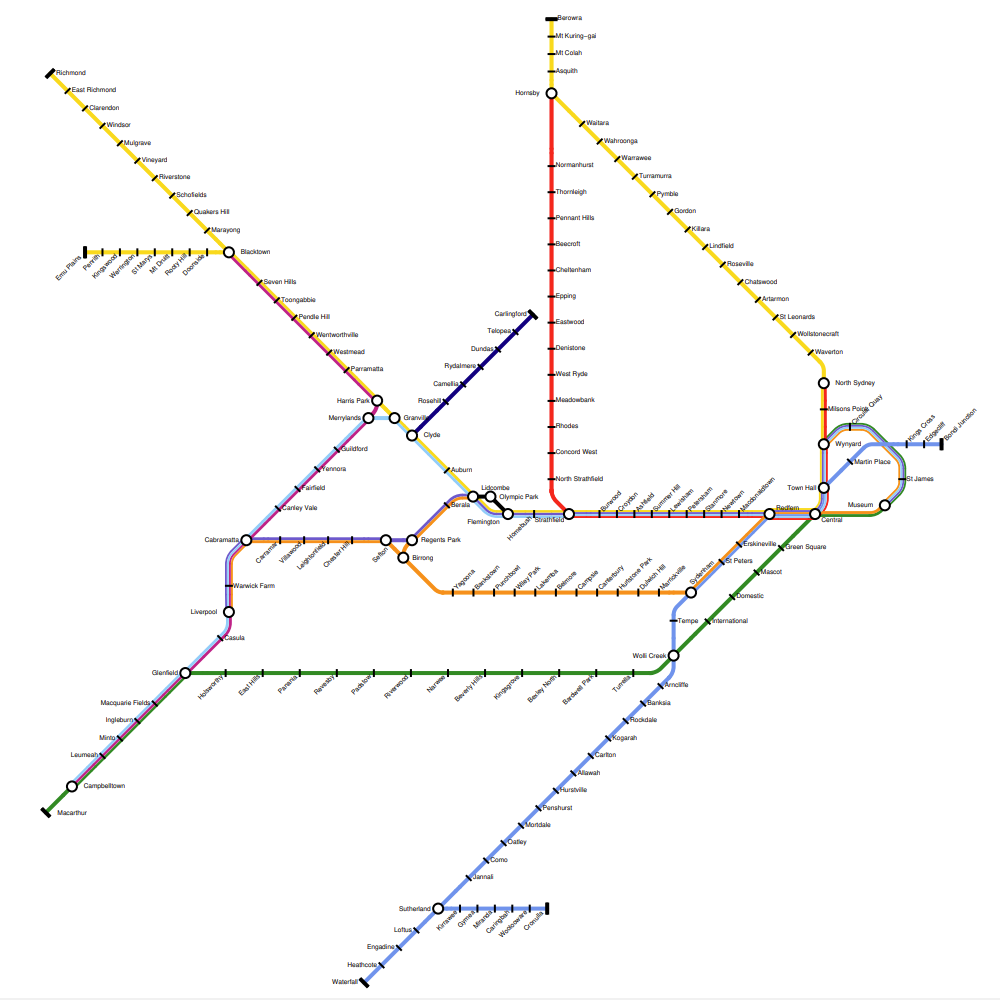
\includegraphics[width=\linewidth]{sydney_nollenburg.png}\\
%       {\scriptsize Layout MIP (Nöllenburg e Wolff)}
%     \end{column}
%   \end{columns}
%   \vspace{0.3cm}
%   \centering
%   {\small Redes de metrô: topologia regular, dezenas a centenas de estações.\\
%   Porto Alegre: malha viária densa, bifurcações não triviais.}
% \end{frame}

% ============================================================
\section{Modelo de Nöllenburg e Wolff}
% ============================================================

\begin{frame}[plain]
  \sectionpage
\end{frame}

\begin{frame}{Modelo MIP de Nöllenburg e Wolff}
  \begin{itemize}
    \item \textbf{Ideia central:} Transformar propriedades desejáveis do mapa em restrições lineares.
    \begin{itemize}
      \item Restrições rígidas \textit{Hard Constraints}
      \item Restrições flexíveis \textit{Soft Constraints} a serem otimizadas
    \end{itemize}
  
    \item \textbf{Propriedades:}
    \begin{itemize}
      \item Octilinearidade
      \item Minimização de curvas
      \item Preservação da posição relativa e da topologia
      \item Uniformidade de tamanho de arestas
    \end{itemize}
  \end{itemize}
\end{frame}


\begin{frame}{Sistema de Coordenadas}
  \begin{columns}[c]
    \begin{column}{0.45\textwidth}
      \centering
      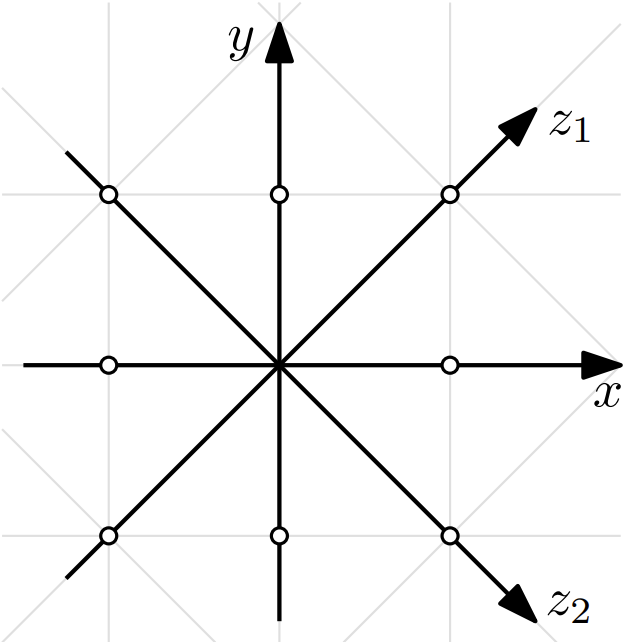
\includegraphics[width=0.85\linewidth]{nollenburg-coords.png}\\
      {\scriptsize Coordenadas octilineares}
    \end{column}
    \begin{column}{0.45\textwidth}
      \centering
      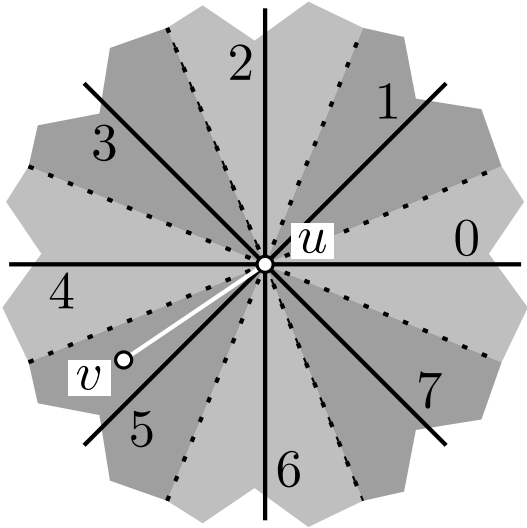
\includegraphics[width=0.85\linewidth]{nollenburg-sec.png}\\
      {\scriptsize 8 setores angulares de 45°}
    \end{column}
  \end{columns}
  \vspace{0.2cm}
  \begin{itemize}
    \item Coordenadas: $(x, y)$ + rotacionadas $z_1, z_2$
    \item $\text{sec}_u(v)$: Setor de $v$ em relação a $u$
  \end{itemize}
\end{frame}

\begin{frame}{Modelo de Nöllenburg: Restrições Rígidas}
  Propriedades obrigatórias que todo layout viável deve satisfazer:

  \vspace{0.25cm}
  \begin{enumerate}
    \item \textbf{Desvio e Octilinearidade}
      \begin{itemize}
        \item \textbf{Variáveis:} Binárias $\alpha_i \in \{0, 1\}$ (3 por aresta) e direções $\text{dir}(v, u)$
        \item \textbf{Complexidade:} $O(|E|)$ variáveis e restrições
      \end{itemize}

    \vspace{0.15cm}
    \item \textbf{Ordem Circular}
      \begin{itemize}
        \item \textbf{Variáveis:} Binárias $\beta_i \in \{0, 1\}$ ($\deg(v)$ por nó)
        \item \textbf{Complexidade:} $O(|E|)$ restrições (espaço de busca escala com $\Delta(G)$)
      \end{itemize}

    \vspace{0.15cm}
    \item \textbf{Não-Cruzamento}
      \begin{itemize}
        \item \textbf{Variáveis:} Binárias $\gamma_i \in \{0, 1\}$ (8 por par de arestas)
        \item \textbf{Complexidade:} \alert{$O(|E|^2)$} restrições e variáveis (principal gargalo)
      \end{itemize}
  \end{enumerate}
\end{frame}

% \begin{frame}{Modelo de Nöllenburg: Desvio e Octilinearidade}
%   Impõe a octilinearidade e abre margem para pequenos desvios relativos
%   \begin{itemize}
%     \item Variáveis binárias $\alpha_i(u,v)$ permitem inclinar a aresta para um setor adjacente:
%   \end{itemize}
%   $$\alpha_{\text{prec}}(u,v) + \alpha_{\text{orig}}(u,v) + \alpha_{\text{succ}}(u,v) = 1$$
%   \begin{itemize}
%     \item Direção final: $\text{dir}(u,v) = \sum_i \text{sec}_i^u(v)\cdot\alpha_i(u,v)$
%     \item Coordenadas forçadas à direção escolhida via \textit{Big-M}, com comprimento mínimo $\ell_{uv}$:
%   \end{itemize}
%   \begin{align*}
%     y(u) - y(v) &\le M(1 - \alpha_{\text{prec}}(u, v)) \\
%     -y(u) + y(v) &\le M(1 - \alpha_{\text{prec}}(u, v)) \\
%     x(u) - x(v) &\ge -M(1 - \alpha_{\text{prec}}(u, v)) + \ell_{uv} \\
%     &\vdots
%   \end{align*}
% \end{frame}

% \begin{frame}{Modelo de Nöllenburg: Ordem Circular}
%   Preserva a ordem cíclica das arestas em torno de cada vértice $v$ ($\deg(v)\ge 2$), mantendo a topologia.

%   \vspace{0.2cm}
%   \begin{itemize}
%     \item Vizinhos $u_1,\dots,u_{\deg(v)}$ ordenados ciclicamente
%     \item Binárias $\beta_i(v)$ escolhem uma permutação cíclica; exatamente uma é ativa:
%   \end{itemize}
%   $$\sum_{i=1}^{\deg(v)} \beta_i(v) = 1$$
%   \begin{itemize}
%     \item As direções devem respeitar a ordem escolhida (módulo 8):
%   \end{itemize}
%   \begin{align*}
%     \text{dir}(v,u_1) &\le \text{dir}(v,u_2) - 1 + 8\,\beta_1(v) \\
%     &\;\;\vdots \\
%     \text{dir}(v,u_{\deg(v)}) &\le \text{dir}(v,u_1) - 1 + 8\,\beta_{\deg(v)}(v)
%   \end{align*}
%   %\alert{Vértices de grau alto restringem possibilidades e aumentam a complexidade} $\Rightarrow$ motivou limitar $\Delta(G)\le 5$.
% \end{frame}

% \begin{frame}{Modelo de Nöllenburg: Não-Cruzamento}
%   Evita cruzamentos entre arestas não adjacentes $e_1=(u_1,v_1)$ e $e_2=(u_2,v_2)$.

%   \vspace{0.2cm}
%   \begin{itemize}
%     \item As arestas devem estar totalmente separadas em ao menos uma das 8 direções (N, S, E, W, NE, NW, SE, SW)
%     \item Binárias $\gamma_i(e_1,e_2)$ selecionam a direção de separação:
%   \end{itemize}
%   $$\sum_{i\in\{\text{N,S,E,W,NE,NW,SE,SW}\}} \gamma_i(e_1,e_2) \ge 1$$
%   \begin{align*}
%     x(u_2) - x(u_1) &\le M\,(1-\gamma_{E}(e_1,e_2)) - d_{\min} \\
%     x(u_2) - x(v_1) &\le M(1 - \gamma_{\text{E}}(e_1, e_2)) - d_{\text{min}}  \\
%     &\;\;\vdots \quad (\text{para as 4 combinações de vértices})
%   \end{align*}
%   \alert{Complexidade $O(|E|^2)$:} $\Rightarrow$ frequentemente desativada em trabalhos que estendem este modelo.
% \end{frame}

\begin{frame}{Modelo de Nöllenburg: Restrições Flexíveis}
  Função objetivo é a combinação linear ponderada de 3 restrições flexíveis:

  \vspace{0.2cm}
  \begin{block}{}
    \centering
    $\displaystyle\min \quad w_{\text{bends}} \cdot C_{\text{bends}} + w_{\text{rpos}} \cdot C_{\text{rpos}} + w_{\text{len}} \cdot C_{\text{len}}$
  \end{block}

  \vspace{0.2cm}
  \begin{itemize}
    \item $C_{\text{bends}}$: custo das \textbf{curvas} nas rotas
    \item $C_{\text{rpos}}$: custo de desvio na \textbf{posição relativa}
    \item $C_{\text{len}}$: custo de \textbf{comprimento} total das arestas
  \end{itemize}

  \vspace{0.3cm}
  \begin{exampleblock}{}
    Pesos $w$ permitem priorizar diferentes critérios estéticos.
  \end{exampleblock}
\end{frame}

% \begin{frame}{Aplicação do Modelo: Sydney}
%   \begin{columns}[c]
%     \begin{column}{0.48\textwidth}
%       \centering
%       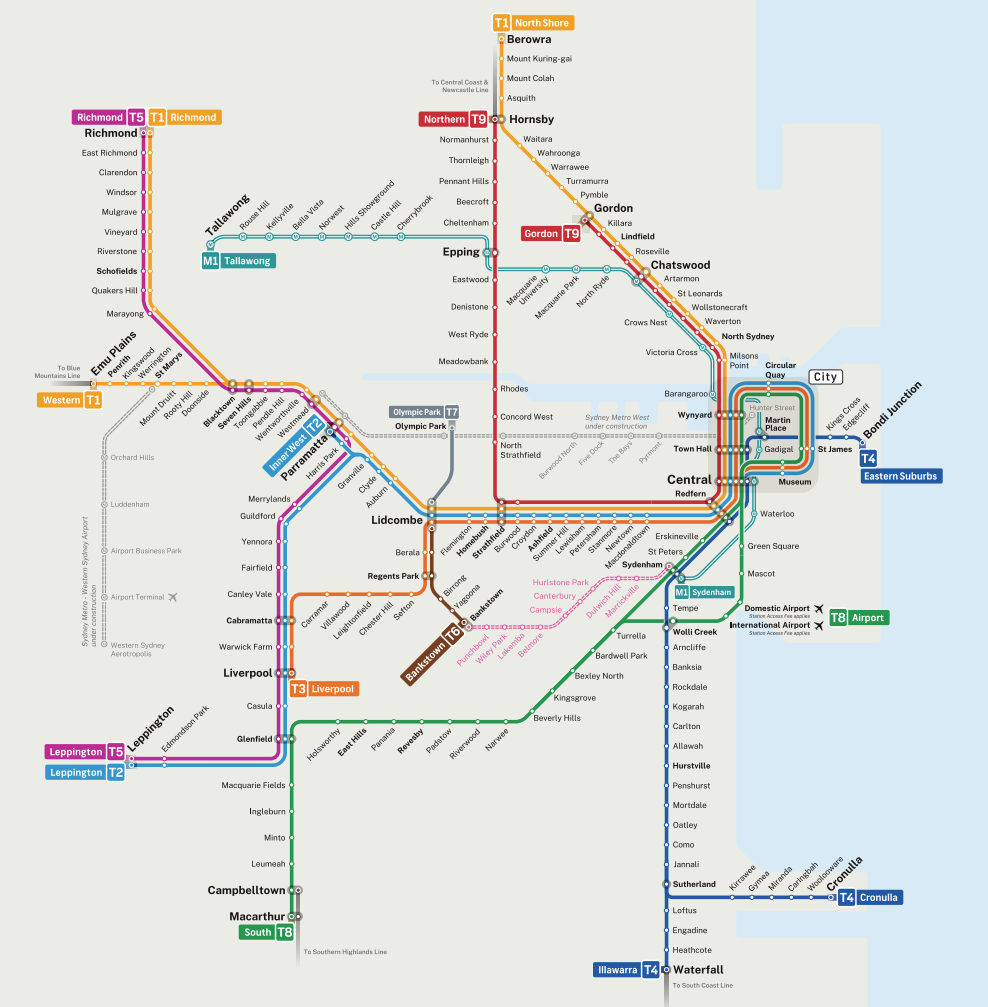
\includegraphics[width=\linewidth]{sydney_original.png}\\
%       {\scriptsize Mapa oficial de Sydney}
%     \end{column}
%     \begin{column}{0.48\textwidth}
%       \centering
%       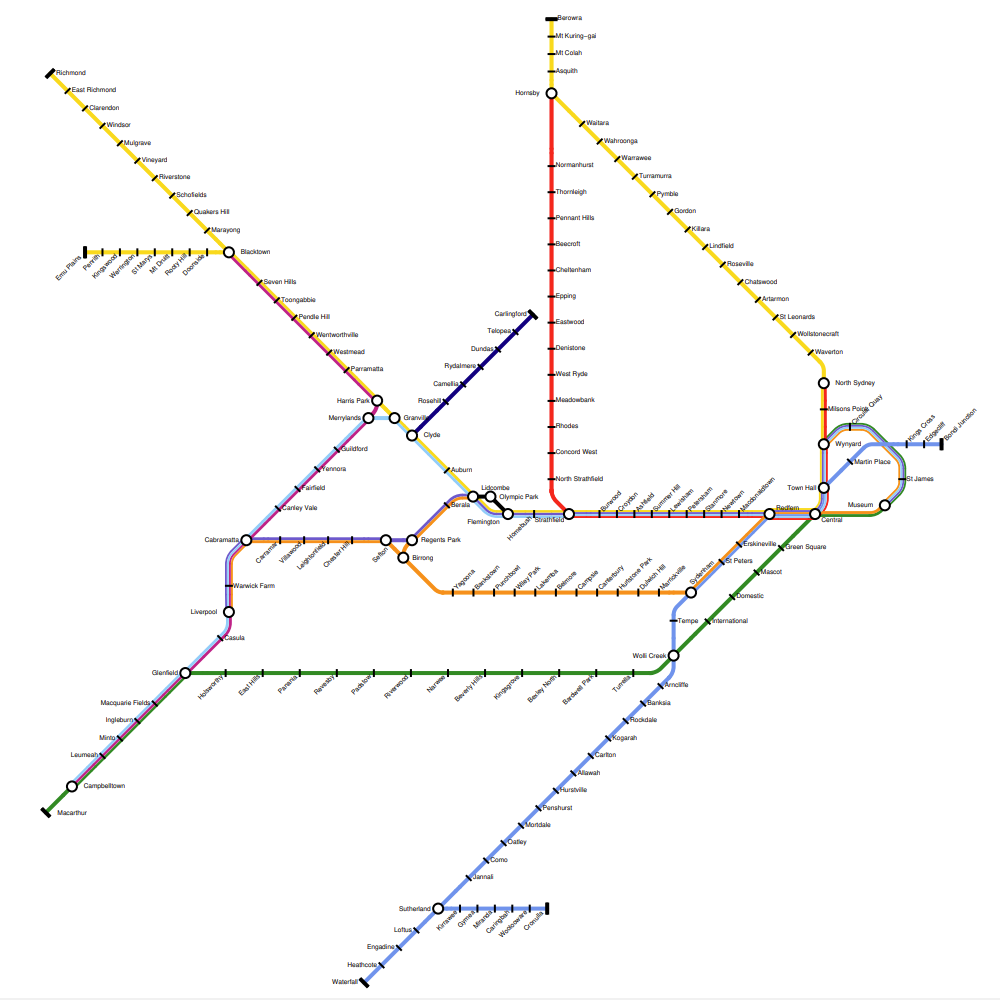
\includegraphics[width=\linewidth]{sydney_nollenburg.png}\\
%       {\scriptsize Layout MIP (Nöllenburg e Wolff)}
%     \end{column}
%   \end{columns}
%   \vspace{0.3cm}
%   \centering
% \end{frame}

% \begin{frame}{Padrão de Dados GTFS}
%   \begin{itemize}
%     \item Dados da EPTC de Porto Alegre
%     \item \textbf{GTFS} (\textit{General Transit Feed Specification}): padrão aberto internacional
%     \item Construção das rotas no grafo via \texttt{stops.txt} ou via \texttt{shapes.txt}
%   \end{itemize}

%   \vspace{0.2cm}
%   \begin{center}
%   \small
%   \begin{tabular}{ll}
%     \toprule
%     \textbf{Arquivo} & \textbf{Informação Principal} \\
%     \midrule
%     \texttt{routes.txt}      & Linhas, nomes, cores \\
%     \texttt{trips.txt}       & Viagens, sentidos, shapes \\
%     \texttt{stops.txt}       & Paradas: nome, lat, lon \\
%     \texttt{stop\_times.txt} & Sequência de paradas por viagem \\
%     \texttt{shapes.txt}      & Geometria: lat, lon  \\
%     \bottomrule
%   \end{tabular}
%   \end{center}
% \end{frame}

% ============================================================
\section{Padrão GTFS}
% ============================================================

\begin{frame}[plain]
  \sectionpage
\end{frame}

\begin{frame}{Padrão de Dados GTFS}
  \begin{itemize}
    \item Dados da EPTC de Porto Alegre
    \item \textbf{GTFS}: padrão internacional para dados geográficos
    \item Construção do grafo via \texttt{stops.txt} ou via \texttt{shapes.txt}
  \end{itemize}
  \vspace{0.2cm}
  \centering
  \resizebox{0.95\textwidth}{!}{%
  \begin{tikzpicture}[
    table_header/.style={
      rectangle, draw=blue!80!black, fill=blue!20, thick,
      minimum width=3.8cm, minimum height=0.65cm,
      font=\bfseries\small, align=center
    },
    table_body/.style={
      rectangle, draw=blue!80!black, fill=blue!3, thick,
      minimum width=3.8cm, minimum height=2.4cm,
      align=left, text width=3.4cm,
      font=\footnotesize\ttfamily, inner sep=5pt
    },
    rel_edge/.style={very thick, gray!75!black},
    card_label/.style={font=\scriptsize\bfseries, text=gray!90!black}
  ]
    % --- LINHA 1 ---
    \node[table_header] (routes_h) at (0, 3.8) {\texttt{routes.txt}};
    \node[table_body, below=0pt of routes_h] (routes_b) {
      \underline{route\_id} \hfill \normalfont\textbf{\scriptsize PK} \\
      route\_short\_name \\
      route\_color
    };

    \node[table_header, fill=orange!25, draw=orange!85!black] (trips_h) at (5.2, 3.8) {\texttt{trips.txt}};
    \node[table_body, fill=orange!5, draw=orange!85!black, below=0pt of trips_h] (trips_b) {
      \underline{trip\_id} \hfill \normalfont\textbf{\scriptsize PK} \\
      route\_id \hfill \normalfont\textit{\scriptsize FK} \\
      shape\_id \hfill \normalfont\textit{\scriptsize FK} \\
      direction\_id
    };

    \node[table_header] (shapes_h) at (10.4, 3.8) {\texttt{shapes.txt}};
    \node[table_body, below=0pt of shapes_h] (shapes_b) {
      \underline{shape\_id} \hfill \normalfont\textbf{\scriptsize PK} \\
      \underline{shape\_pt\_sequence} \hfill \normalfont\textbf{\scriptsize PK} \\
      shape\_pt\_lat \\
      shape\_pt\_lon
    };

    % --- LINHA 2 ---
    \node[table_header] (stops_h) at (0, -0.4) {\texttt{stops.txt}};
    \node[table_body, below=0pt of stops_h] (stops_b) {
      \underline{stop\_id} \hfill \normalfont\textbf{\scriptsize PK} \\
      stop\_name \\
      stop\_lat \\
      stop\_lon
    };

    \node[table_header, fill=teal!25, draw=teal!85!black] (stoptimes_h) at (5.2, -0.4) {\texttt{stop\_times.txt}};
    \node[table_body, fill=teal!5, draw=teal!85!black, below=0pt of stoptimes_h] (stoptimes_b) {
      \underline{trip\_id} \hfill \normalfont\textbf{\scriptsize PK, FK} \\
      \underline{stop\_sequence} \hfill \normalfont\textbf{\scriptsize PK} \\
      stop\_id \hfill \normalfont\textit{\scriptsize FK}
    };

    % --- RELACIONAMENTOS ---
    \draw[rel_edge] (routes_b.east) -- (trips_b.west |- routes_b.east)
      node[card_label, very near start, above=1pt] {1}
      node[card_label, very near end, above=1pt] {N};
    \draw[rel_edge] (shapes_b.west) -- (trips_b.east |- shapes_b.west)
      node[card_label, very near start, above=1pt] {1}
      node[card_label, very near end, above=1pt] {N};
    \draw[rel_edge] (trips_b.south) -- (stoptimes_h.north -| trips_b.south)
      node[card_label, very near start, right=1pt] {1}
      node[card_label, very near end, right=1pt] {N};
    \draw[rel_edge] (stops_b.east) -- (stoptimes_b.west |- stops_b.east)
      node[card_label, very near start, above=1pt] {1}
      node[card_label, very near end, above=1pt] {N};
  \end{tikzpicture}%
  }
\end{frame}

% \begin{frame}{Arquitetura da Solução}
%   \centering
%   \resizebox{0.95\textwidth}{!}{%
%   \begin{tikzpicture}[
%     node distance=1.0cm and 1.2cm,
%     io/.style={trapezium, trapezium left angle=70, trapezium right angle=110, minimum width=2cm, minimum height=0.8cm, text centered, text width=2cm, draw=black, fill=green!15, font=\small},
%     modulo/.style={rectangle, rounded corners, minimum width=3cm, minimum height=1cm, text centered, text width=2.8cm, draw=black, fill=blue!15, font=\small},
%     modulo_main/.style={rectangle, rounded corners, minimum width=2.5cm, minimum height=1cm, text centered, text width=2.5cm, draw=black, fill=orange!20, very thick, font=\small},
%     solver/.style={rectangle, rounded corners, minimum width=2.2cm, minimum height=1cm, text centered, draw=black, fill=red!15, font=\small},
%     seta/.style={-Stealth, very thick}
%   ]
%     \node (gtfs) [io] {Dados GTFS};
%     \node (parser) [modulo, right=of gtfs] {\texttt{data\_parser.jl} \\ {\scriptsize Pré-processamento}};
%     \node (map) [modulo_main, right=of parser] {\texttt{map.jl} \\ {\scriptsize Orquestrador}};
%     \node (export) [modulo, right=of map] {\texttt{gtfs\_to\_xml.jl} \\ {\scriptsize Exportação}};
%     \node (graphml) [io, right=of export] {GraphML};

%     \node (mip) [modulo, minimum width=3.8cm, text width=3.6cm, above=of map] {\texttt{mip\_constraints.jl} \\ {\scriptsize Modelo MIP}};
%     \node (cplex) [solver, below=of map, yshift=-0.1cm] {Solver CPLEX};

%     \draw[seta] (gtfs) -- (parser);
%     \draw[seta] (parser) -- (map);
%     \draw[seta] (map) -- (export);
%     \draw[seta] (export) -- (graphml);
%     \draw[seta] (mip.south) -- (map.north);
%     \draw[seta] (cplex.north) -- (map.south);
%   \end{tikzpicture}%
%   }

%   \vspace{0.4cm}
%   \begin{itemize}
%     \item Linguagem \textbf{Julia} + solver \textbf{IBM CPLEX} (JuMP.jl)
%     \item Visualização: GUI Java de Nöllenburg (JUNG + GraphML)
%   \end{itemize}
% \end{frame}


% ============================================================
\section{Construção do Grafo Base}
% ============================================================

\begin{frame}[plain]
  \sectionpage
\end{frame}

\begin{frame}{Dilema: Grafo de Paradas vs.\ Grafo de Traçados}
  \begin{columns}[c]
    \begin{column}{0.42\textwidth}
      \centering
      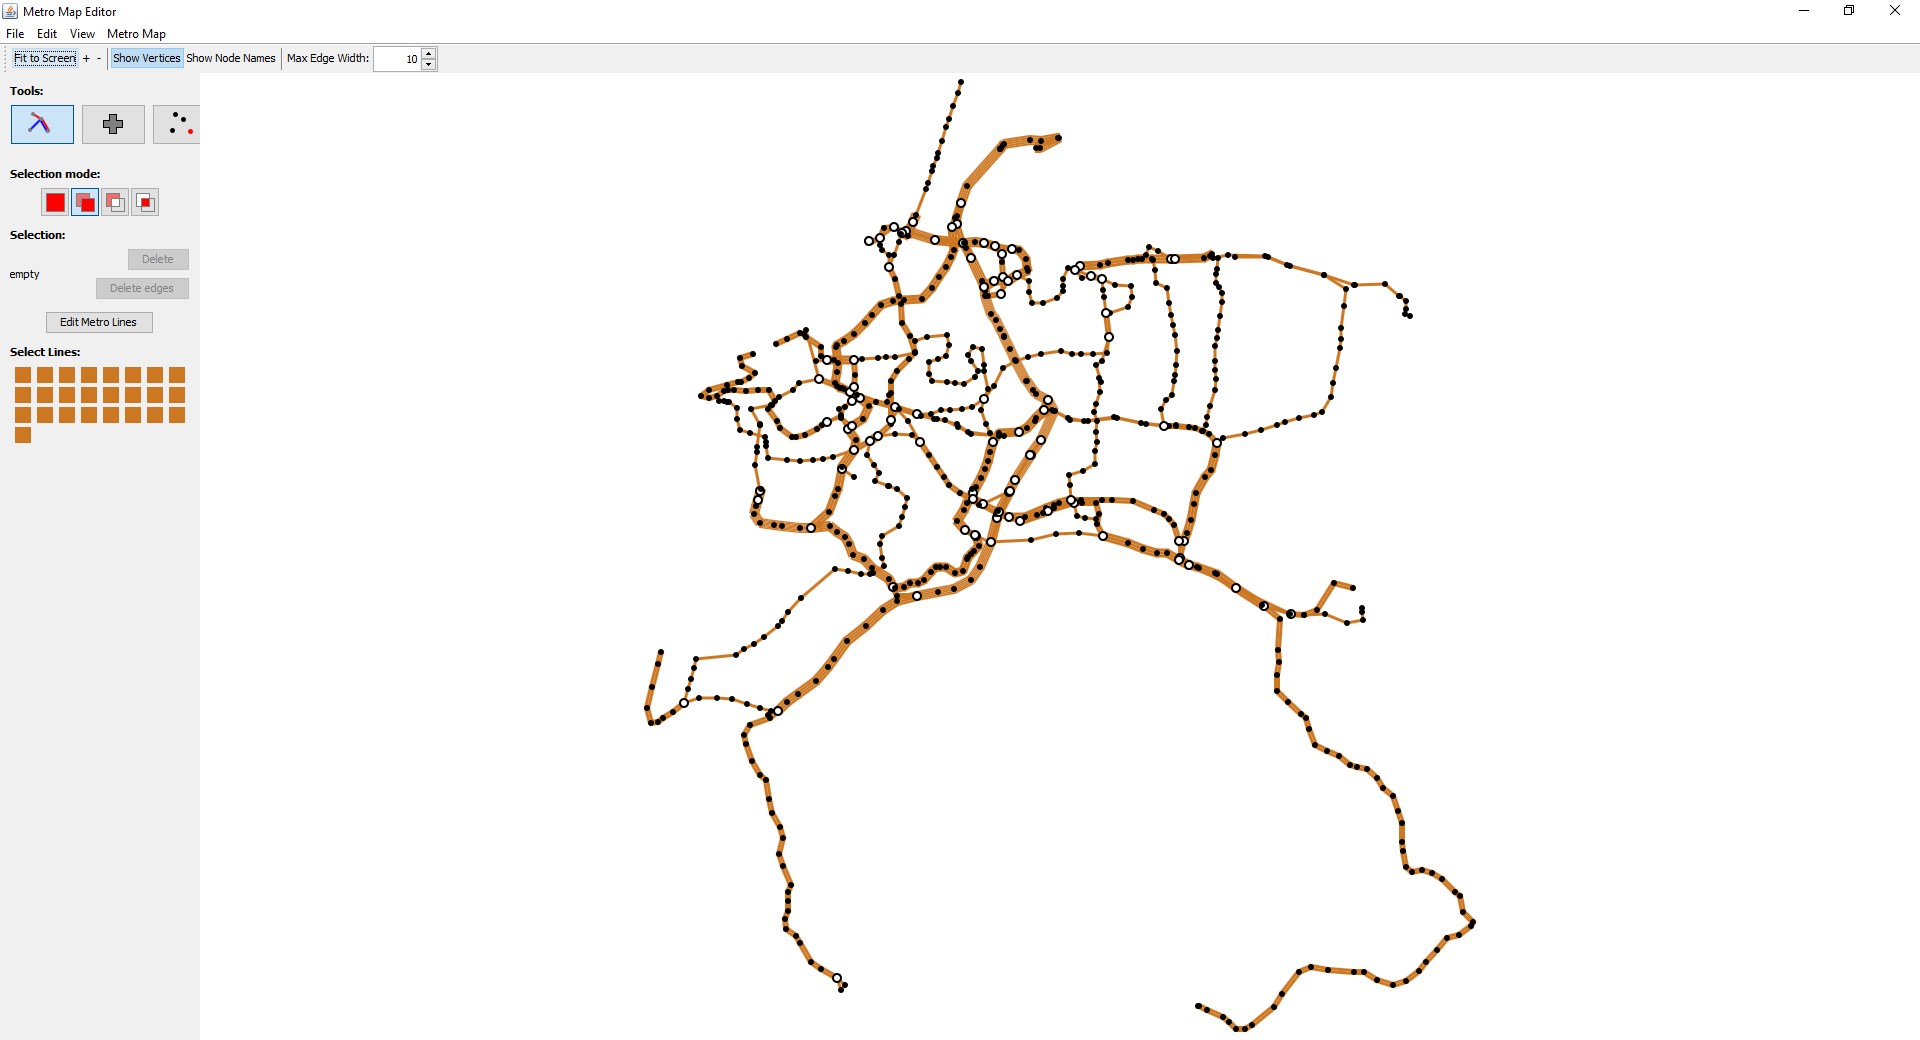
\includegraphics[width=\linewidth, trim=480 0 320 60, clip]{mapa_paradas.png}\\
      {\scriptsize Grafo de Paradas (\texttt{stops})}
    \end{column}
    \begin{column}{0.42\textwidth}
      \centering
      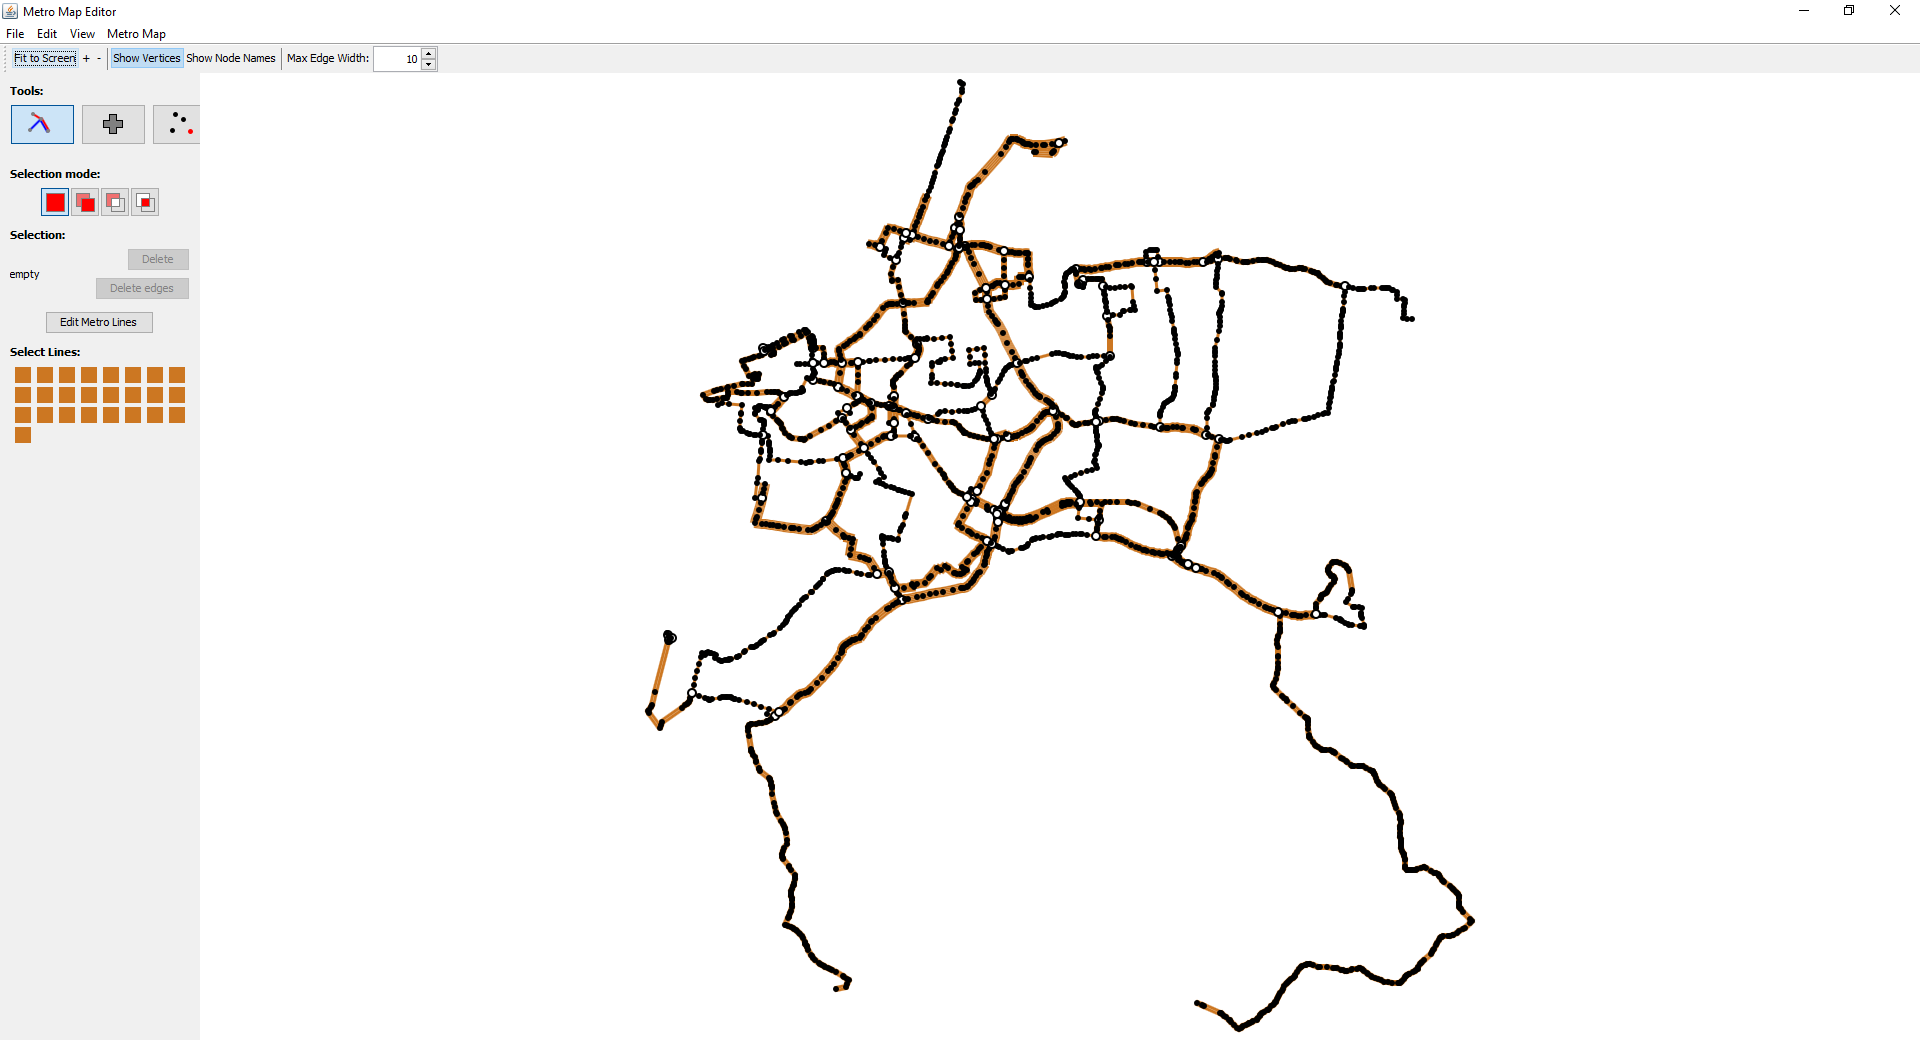
\includegraphics[width=\linewidth, trim=480 0 320 60, clip]{mapa_tracado.png}\\
      {\scriptsize Grafo de Traçado (\texttt{shapes})}
    \end{column}
  \end{columns}
  \vspace{0.2cm}
  \begin{itemize}
    \item \textbf{Paradas:} Vértices de grau até 8, inviável para MIP octilinear
    \item \textbf{Shapes:} Graus menores, mas sem informação de paradas
    \item \textbf{Solução:} Grafo Híbrido — topologia viária + semântica operacional
  \end{itemize}
\end{frame}

\begin{frame}{Construção do Grafo Híbrido}
  \begin{enumerate}
    \item Construir grafos independentes: \texttt{stops} e \texttt{shapes}
    \item Projeção ortogonal das paradas sobre arestas do traçado
    \item \textbf{Priorização semântica:} preferência por arestas que compartilham rotas
    \item Contração de vértices \texttt{shapes} de grau 2
  \end{enumerate}

  \vspace{0.3cm}
  \centering
  \begin{tikzpicture}
    \node[draw=gray!45, fill=gray!15, rounded corners=3pt, inner xsep=8pt, inner ysep=4pt, text width=0.92\linewidth, align=left] {
      \textbf{Resultado:} Taxa acumulativa de retenção de paradas nas rotas: $\mathbf{92{,}89\%}$
    };
  \end{tikzpicture}
  % \centering
  % 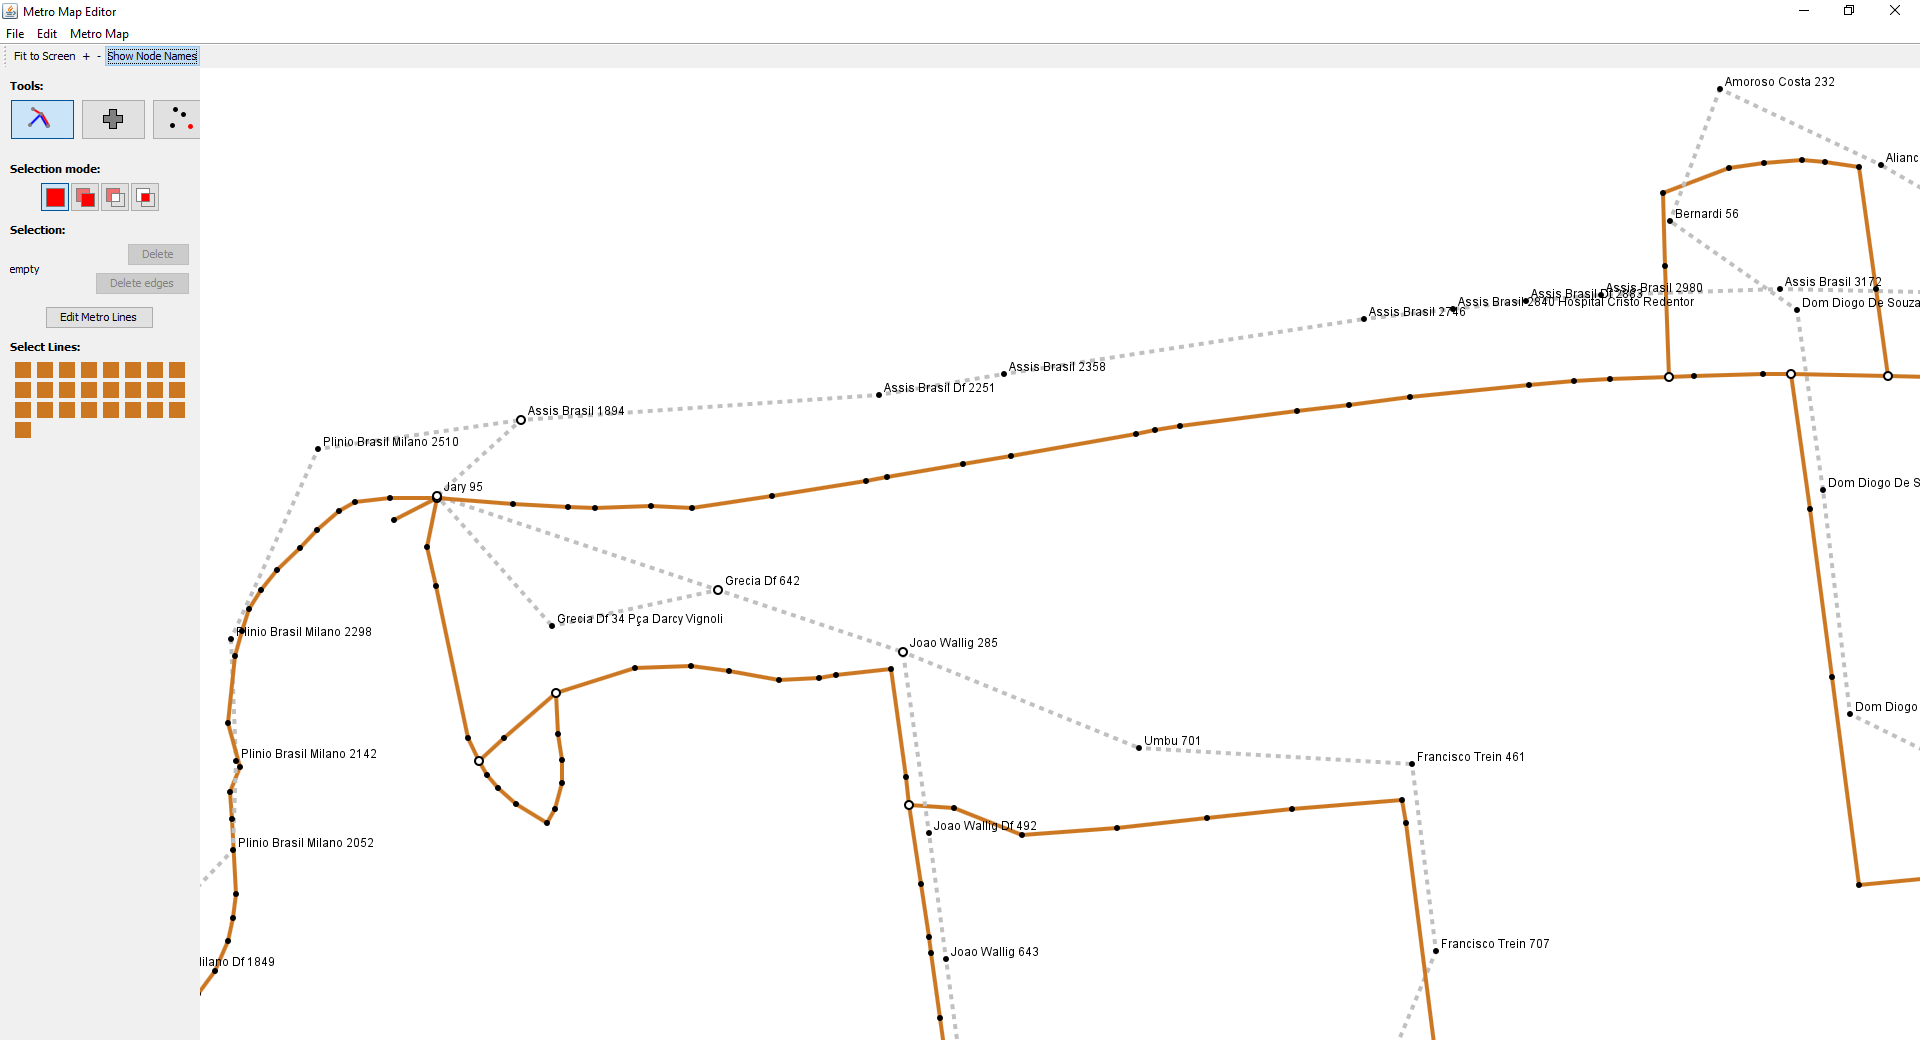
\includegraphics[width=0.7\linewidth, trim=160 0 300 200, clip]{mapa_compara_tracado_parada.png}
\end{frame}

\begin{frame}{Construção do Grafo Híbrido: visualização}
  \centering
  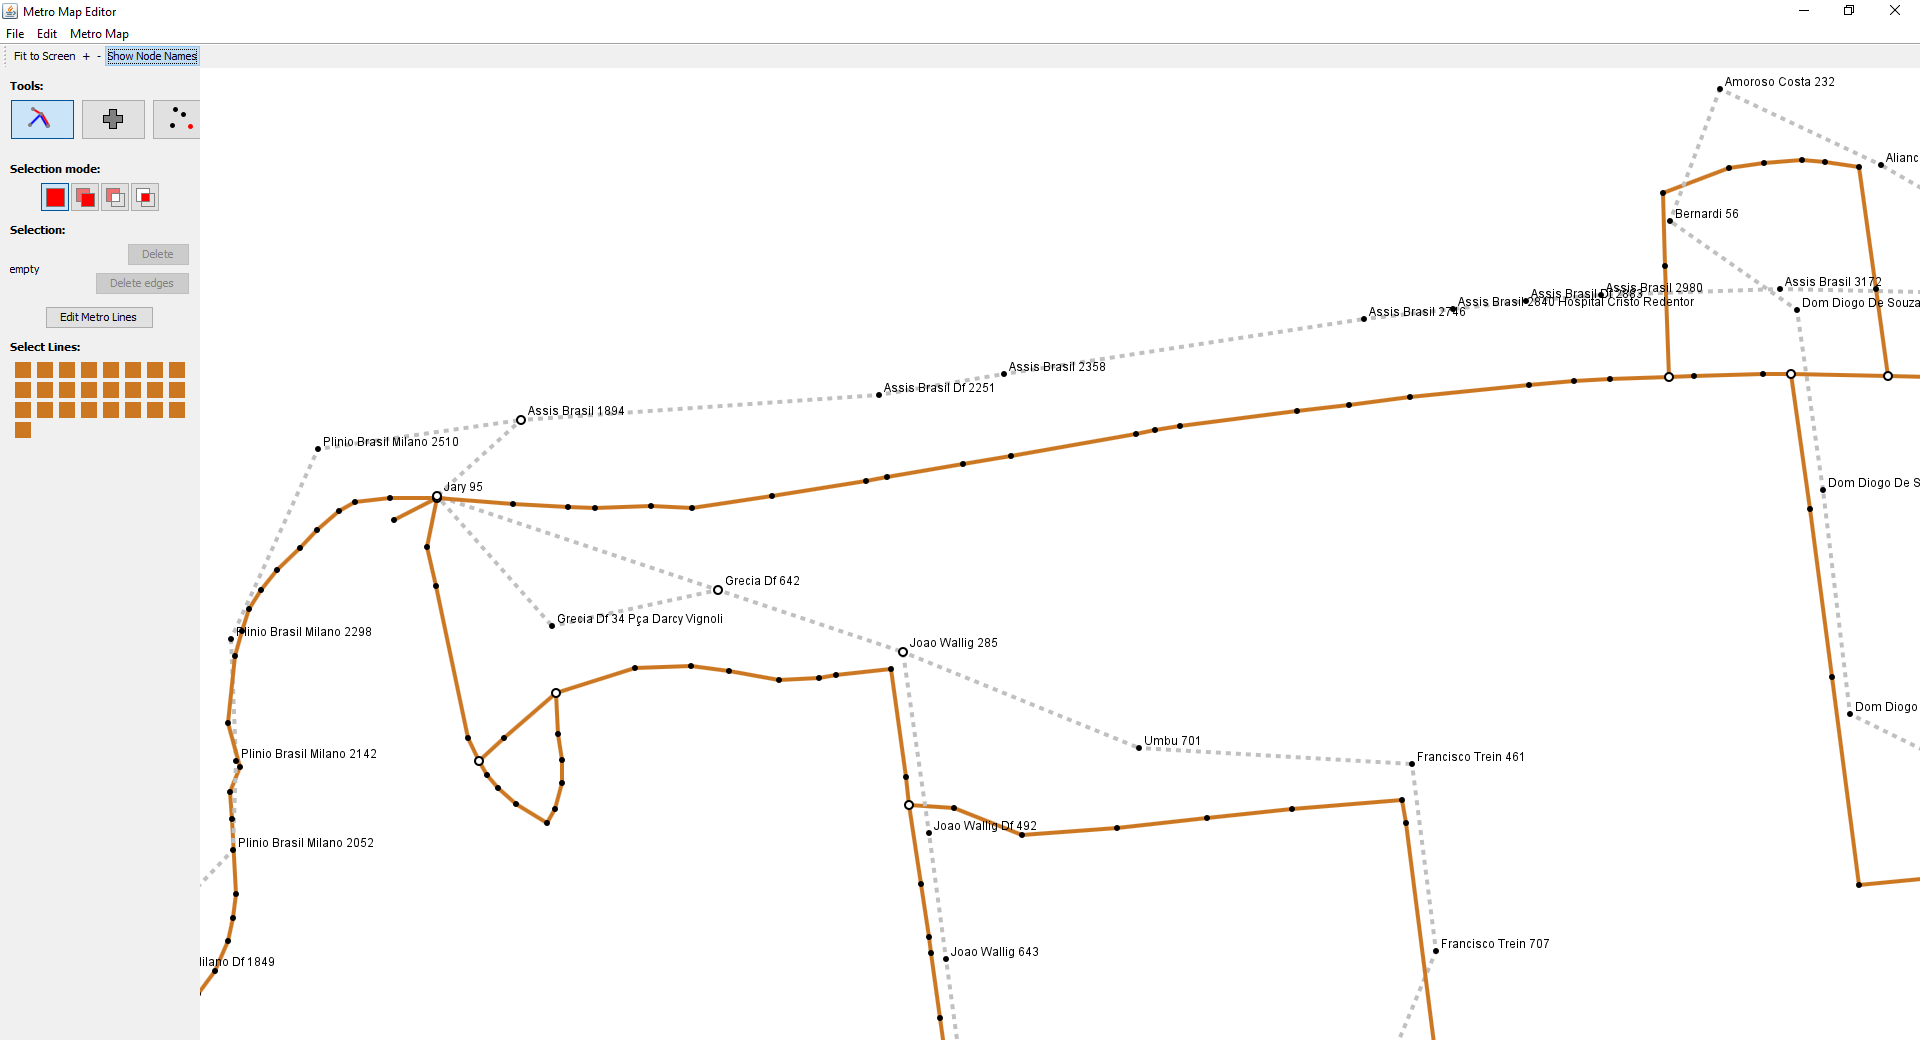
\includegraphics[width=0.9\linewidth, trim=160 0 300 200, clip]{mapa_compara_tracado_parada.png}
\end{frame}

\section{Simplificação do Mapa}

\begin{frame}[plain]
  \sectionpage
\end{frame}

\begin{frame}{Simplificações: Projeção e Fusão}
  Simplifica o traçado visual, reduzindo a escala do grafo e mitigando nós de maior grau de incidência

  \vspace{0.2cm}
  \begin{columns}[T]
    \begin{column}{0.48\textwidth}
      \textbf{1. Projeção Ortogonal}
      \begin{itemize}
        \item Projeta a parada $P$ ortogonalmente sobre a aresta $(U,V)$ se $d \le D_{\text{snap}}$
        \item Substitui $(U,V)$ por $(U,P)$ e $(P,V)$
      \end{itemize}
      \centering
      \vspace{0.15cm}
      \begin{tikzpicture}[
        node_style/.style={circle, draw, fill=blue!20, minimum size=0.6cm, inner sep=1pt, font=\scriptsize\bfseries},
        edge_style/.style={very thick}
      ]
        \node[node_style] (U) at (0,1.3) {U};
        \node[node_style] (V) at (3.0,1.3) {V};
        \node[node_style, fill=red!25] (P) at (1.5,0.3) {P};
        \draw[edge_style] (U) -- (V);
        \draw[dashed, red!80!black, -Latex, thick] (P) -- (1.5,1.3) node[midway, right, font=\tiny] {$d \le D_{\text{snap}}$};
      \end{tikzpicture}
    \end{column}

    \begin{column}{0.48\textwidth}
      \textbf{2. Fusão de Paradas (Merge)}
      \begin{itemize}
        \item Agrupa paradas com distância euclidiana $< D_{\text{merge}}$
        \item Vértice unificado herda todas as conexões e linhas
      \end{itemize}
      \centering
      \vspace{0.15cm}
      \begin{tikzpicture}[
        node_style/.style={circle, draw, fill=blue!20, minimum size=0.6cm, inner sep=1pt, font=\scriptsize\bfseries},
        aura/.style={circle, draw, dashed, gray, thick},
        edge_style/.style={very thick}
      ]
        \node[node_style, fill=red!25] (P1) at (0,0) {P};
        \node[aura, minimum size=2.5cm] at (0,0) {};
        \node[node_style] (P2) at (30:0.85cm) {U};
        \node[node_style] (P3) at (150:1.85cm) {V};
        \draw[edge_style] (P1) -- (P2);
        \draw[edge_style] (P2) -- (P3);
        \node[text=gray!90!black, font=\tiny, above] at (0,1.15cm) {Raio $D_{\text{merge}}$};
      \end{tikzpicture}
    \end{column}
  \end{columns}
\end{frame}

% \begin{frame}{Fusão de Paradas: Exemplo}
%   \begin{columns}[c]
%     \begin{column}{0.4\textwidth}
%       \centering
%       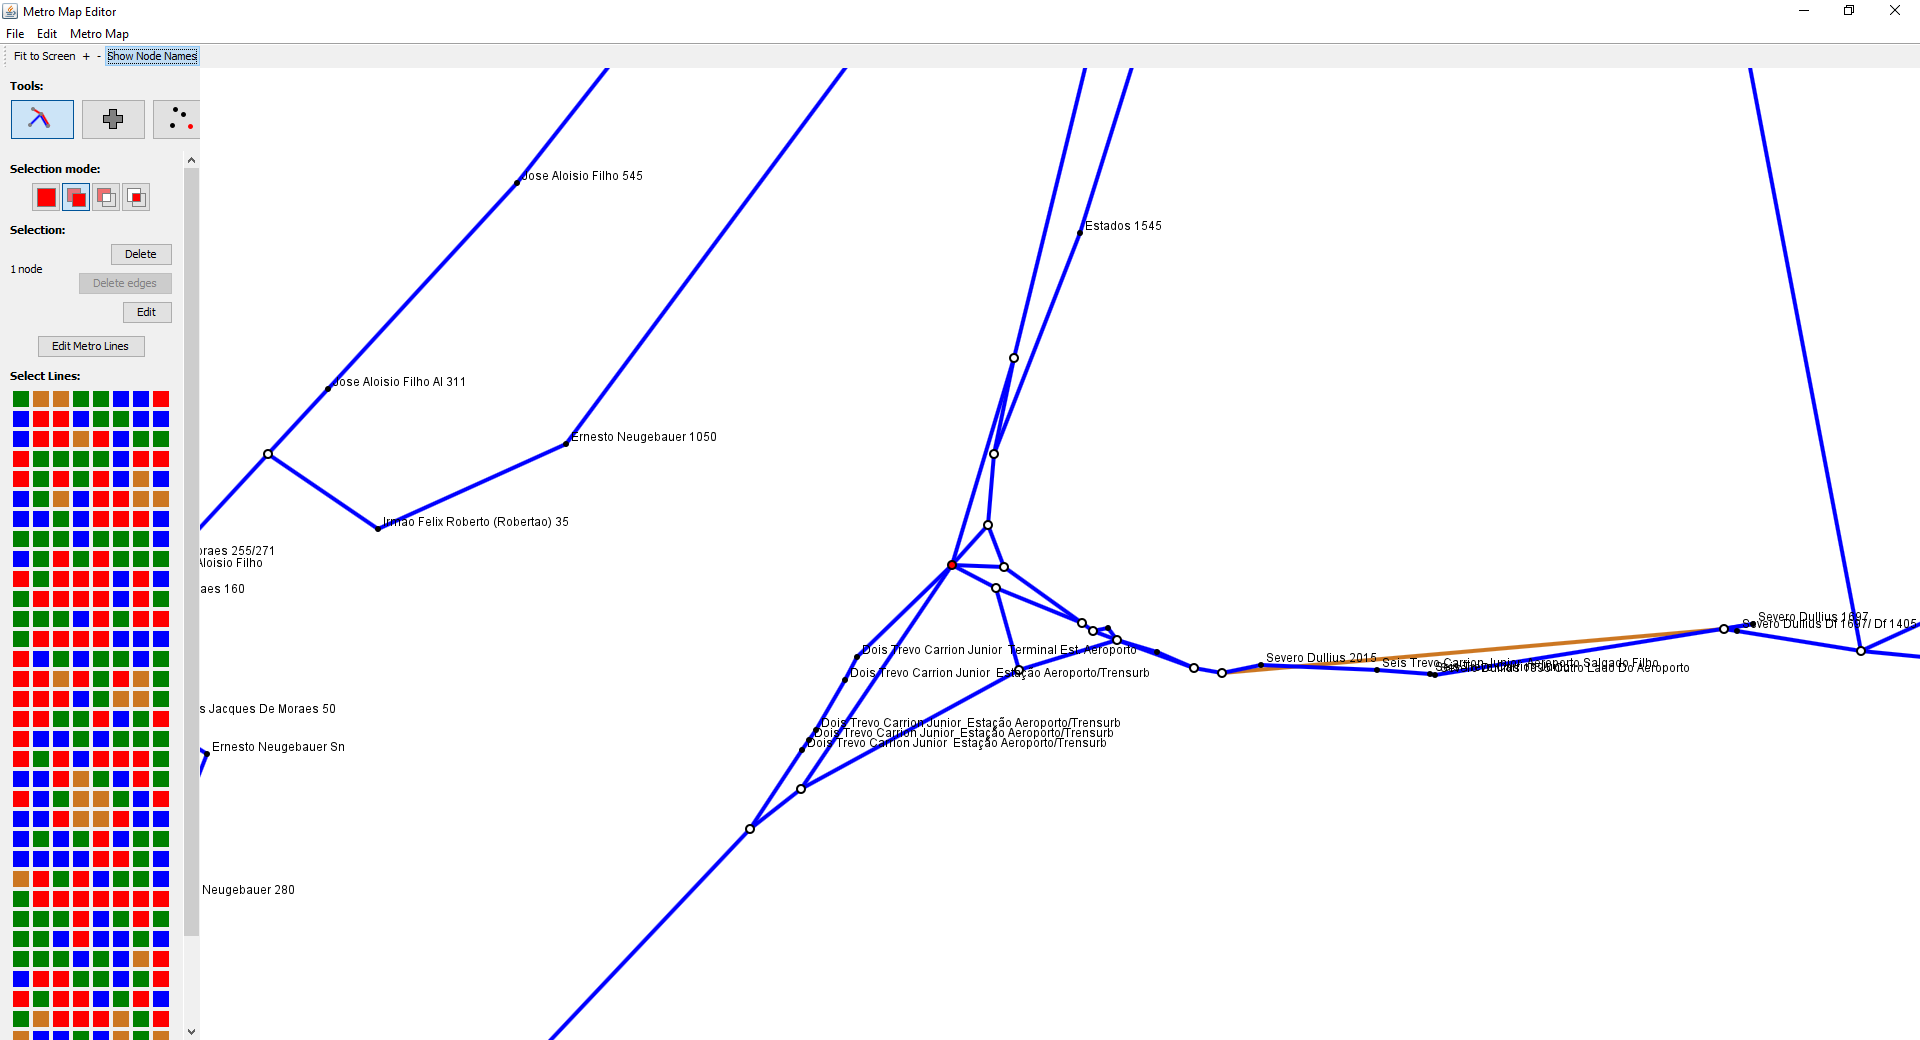
\includegraphics[width=\linewidth, trim=558 100 560 160, clip]{abstracao_antes.png}\\
%       {\scriptsize Antes da fusão}
%     \end{column}
%     \begin{column}{0.4\textwidth}
%       \centering
%       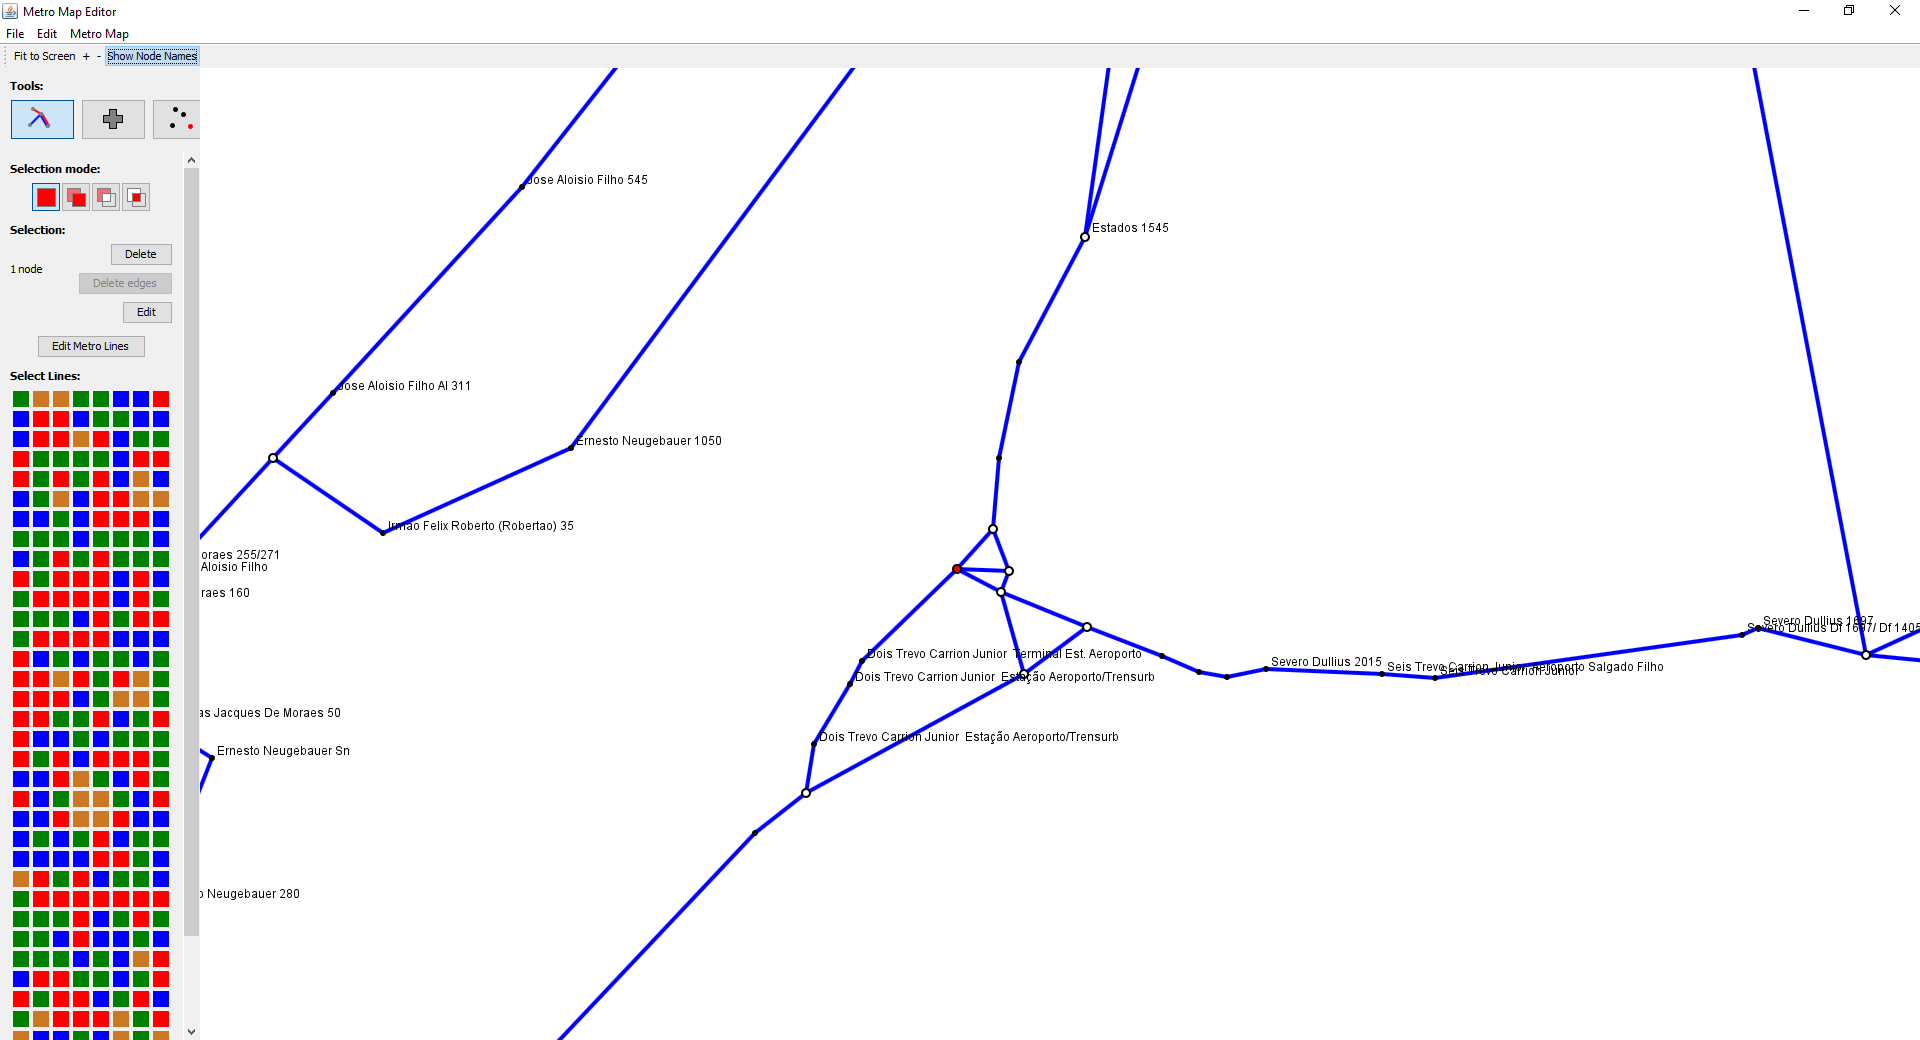
\includegraphics[width=\linewidth, trim=562 100 560 160, clip]{abstracao_depois.png}\\
%       {\scriptsize Depois da fusão}
%     \end{column}
%   \end{columns}
% \end{frame}

\begin{frame}{Simplificações: Remoção de Paradas Adjacentes}
  
  \textbf{3. Remoção de paradas adjacentes por critério angular}
  
  \begin{itemize}
    \item Ângulo de inflexão $\varphi$, remove se $\varphi < 80^\circ$ ou $\varphi > 150^\circ$, preserva curvas que definem o mapa mental do usuário
    \item Vértices removidos são adicionados de volta no pós-processamento
  \end{itemize}
  \vspace{0.3cm}
  \begin{columns}[c]
    \begin{column}{0.3\textwidth}
      \centering
      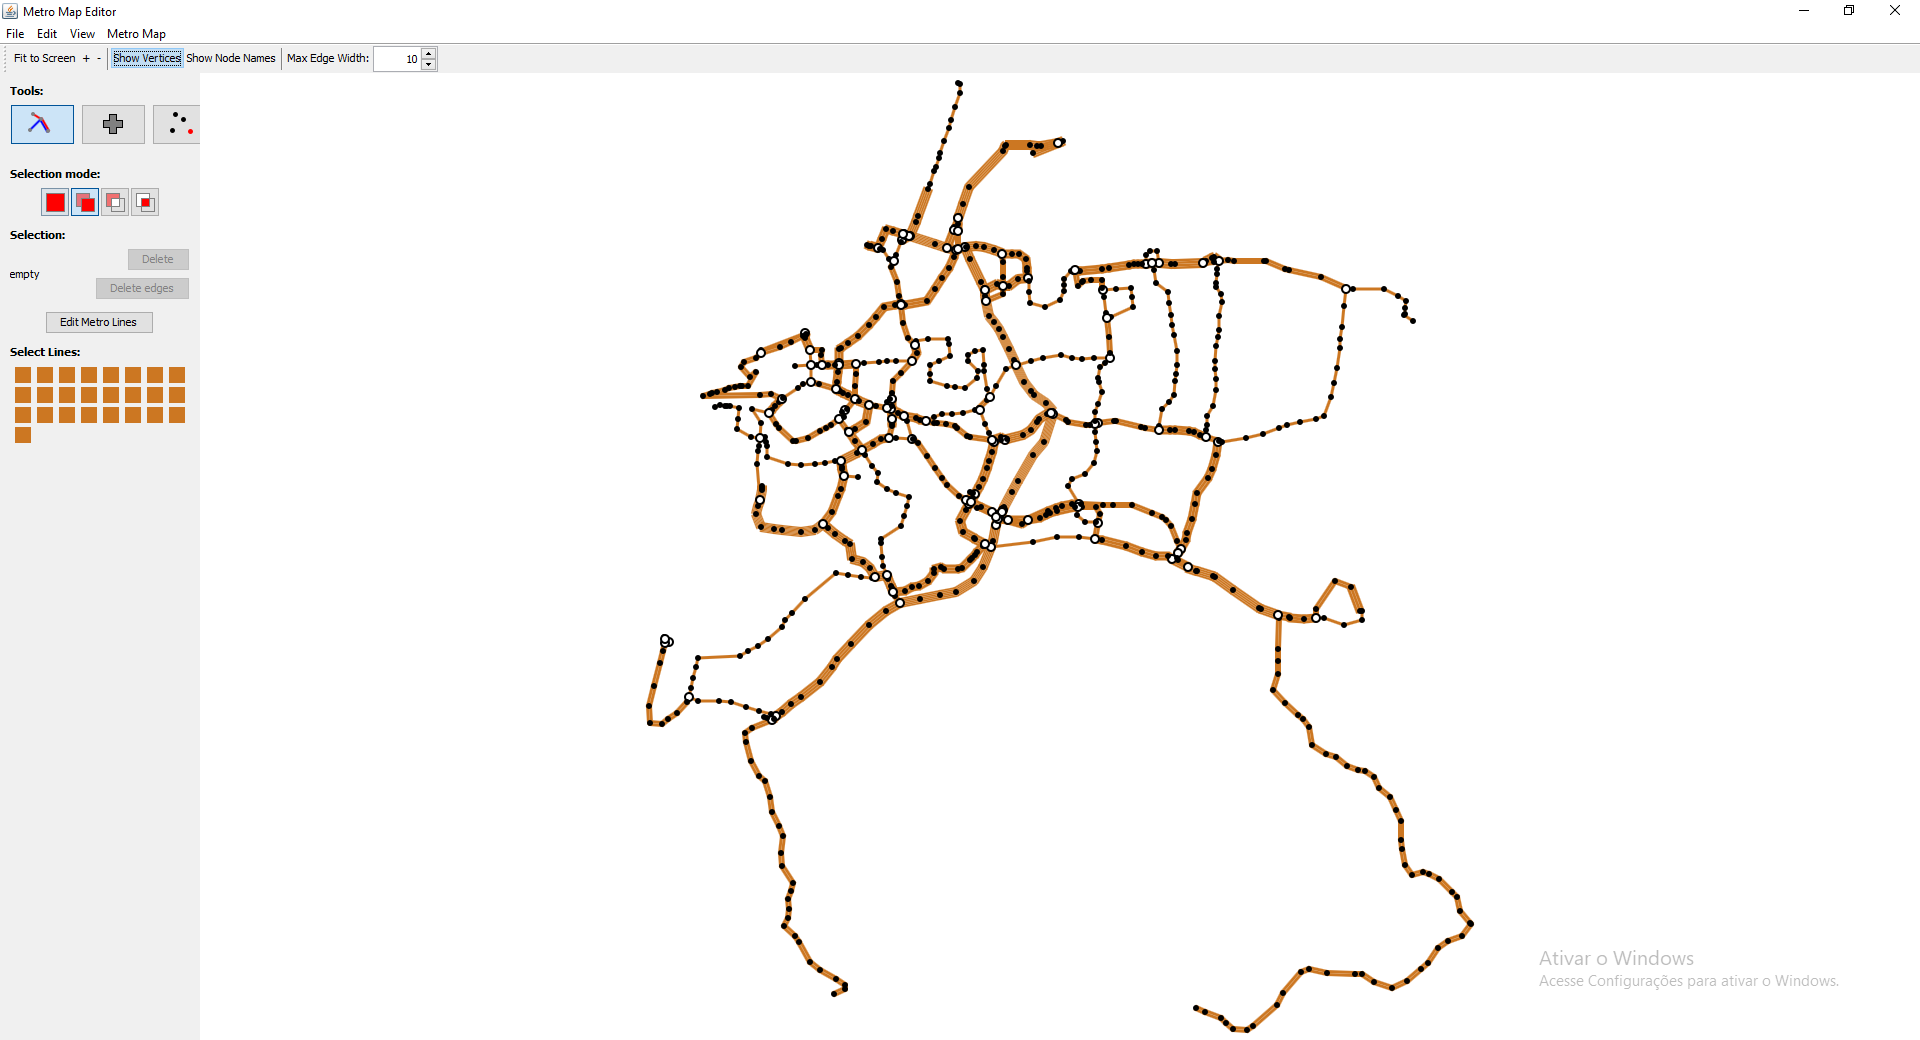
\includegraphics[width=\linewidth, trim=450 0 330 60, clip]{adjacentes_antes.png}\\
      {\scriptsize Original}
    \end{column}
    \begin{column}{0.3\textwidth}
      \centering
      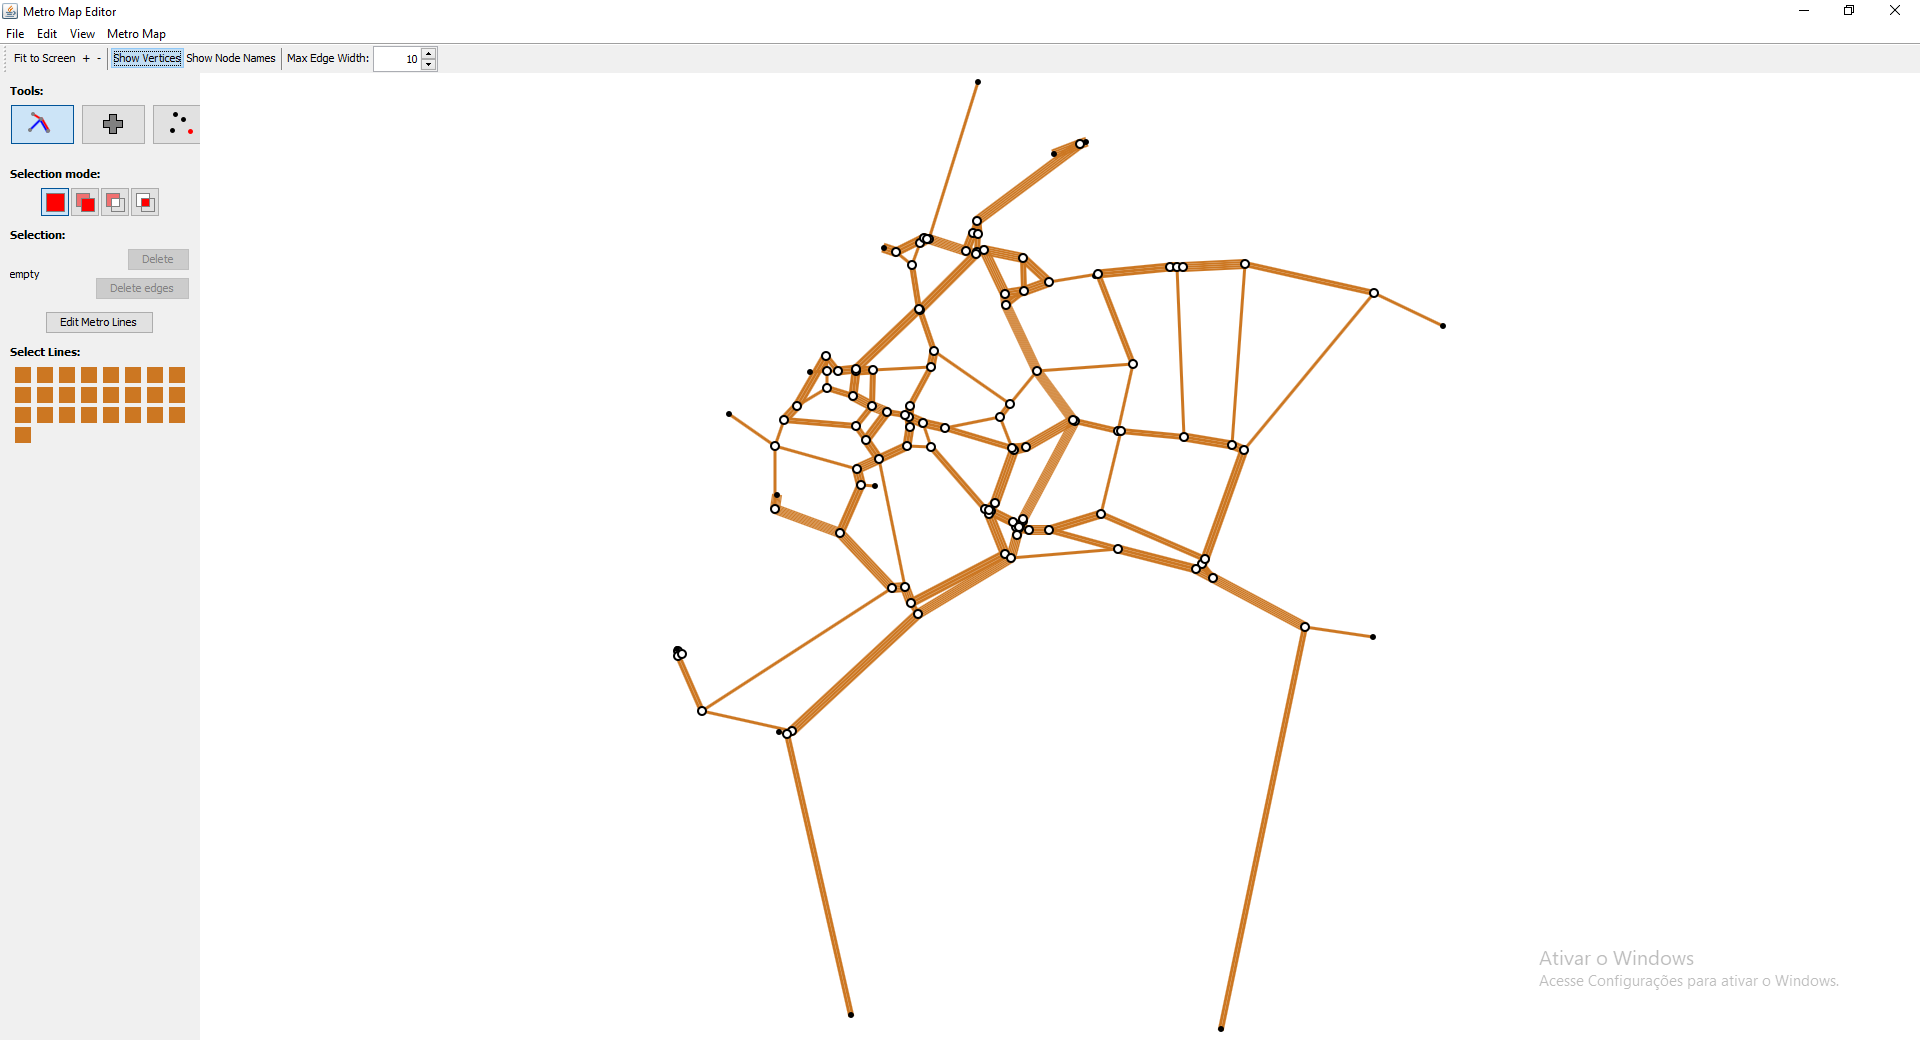
\includegraphics[width=\linewidth, trim=450 0 330 60, clip]{adjacentes_tudo.png}\\
      {\scriptsize Remoção total}
    \end{column}
    \begin{column}{0.3\textwidth}
      \centering
      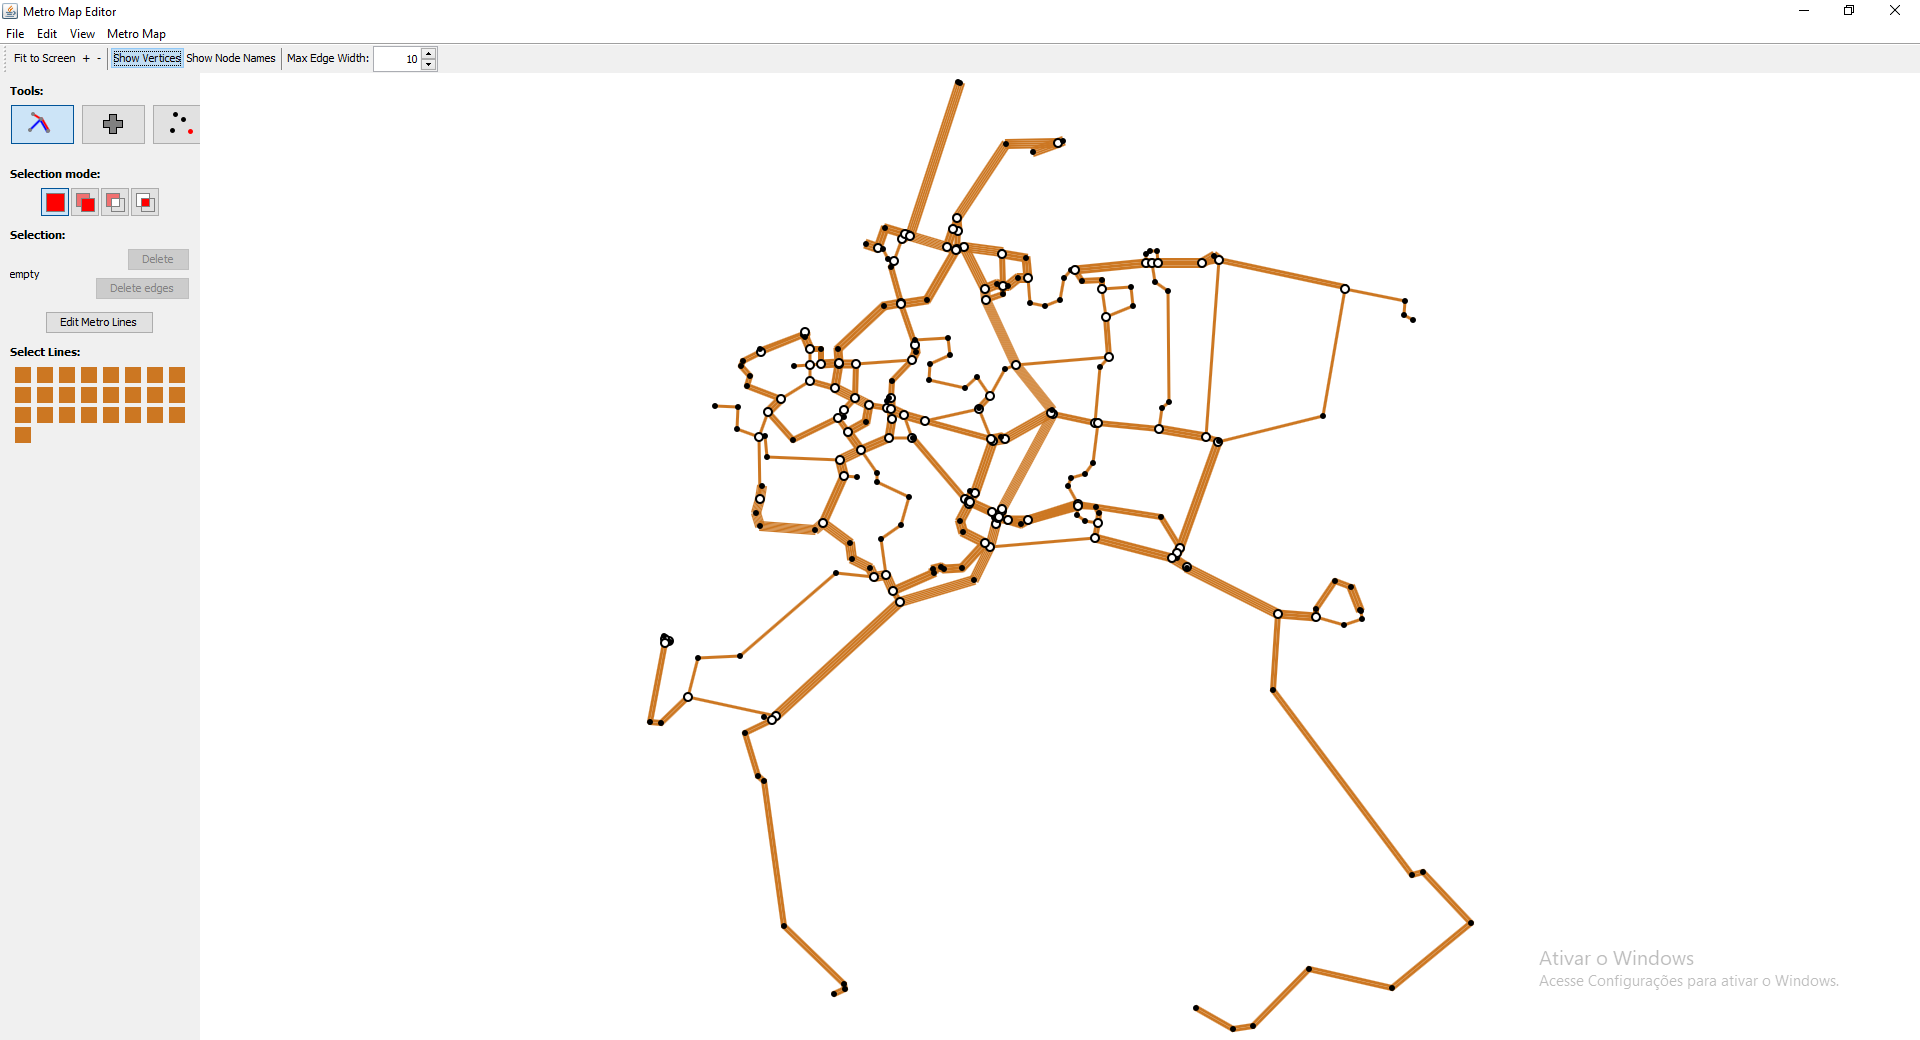
\includegraphics[width=\linewidth, trim=450 0 330 60, clip]{adjacentes_limiar.png}\\
      {\scriptsize Remoção por limiar}
    \end{column}
  \end{columns}
\end{frame}

\begin{frame}{Impacto da Abstração}
  \centering
  \small
  \begin{tabular}{lrrrr}
    \toprule
    \textbf{Etapa} & \textbf{$|V|$} & \textbf{$|E|$} & $\boldsymbol{\Delta(G)}$ & \textbf{Nós $> 4$} \\
    \midrule
    Grafo de Paradas            & 3.831 & 4.382 & 8 & 61 \\
    Grafo Híbrido               & 4.858 & 5.368 & 6 & 5 \\
    Pós Projeção e Fusão        & 4.174 & 4.660 & \textbf{5} & \textbf{3} \\
    Pós Rem. Adjacentes         & \textbf{1.603} & \textbf{2.071} & \textbf{5} & \textbf{3} \\
    \bottomrule
  \end{tabular}

  \vspace{0.3cm}
  \begin{itemize}
    \item Redução de $\mathbf{58\%}$ nos vértices (3.831 $\to$ 1.603)
    \item Grau máximo: $8 \to 5$ — viabiliza permutações e reduz complexidade
  \end{itemize}
\end{frame}

\section{Adaptações do Modelo MIP}

\begin{frame}[plain]
  \sectionpage
\end{frame}

\begin{frame}{Correção Iterativa de Distorções}
  \textbf{Problema:} Sem restrições de cruzamento, a topologia do grafo pode ser distorcida.

  \vspace{0.2cm}
  \textbf{Solução: Correção iterativa}
  \begin{enumerate}
    \item Resolver MIP sem restrições de cruzamento
    \item Detectar pares de vértices não adjacentes com desvio angular $|\Delta\theta| > 100^\circ$ vs.\ orientação original
    \item Adicionar restrições corretivas lineares sob demanda
    \item Reotimizar e repetir até estabilização
  \end{enumerate}

  % \vspace{0.2cm}
  % \textbf{Resultado:} Impacto mínimo no tempo computacional; milhares de correções aplicadas de forma incremental.
\end{frame}

\begin{frame}{Simplificações de Oke e Siddiqui}
  Oke e Siddiqui estendem o modelo com foco em reduzir o espaço de busca e o tempo computacional do modelo original proposto por Nöllenburg e Wolff.

  \vspace{0.2cm}
  \begin{itemize}
    \item \textbf{Relaxação de Coordenadas para $\mathbb{R}$:}
      \begin{itemize}
        \item $x(v), y(v) \in \mathbb{R}$ tornam-se variáveis contínuas (não inteiras)
        \item Transforma modelo em Programa Linear Misto Binário $\Rightarrow$ Evita ramificações de coordenadas no \textit{Branch-and-Bound}
      \end{itemize}

    \item \textbf{Formulação Biobjetiva:}
      \begin{itemize}
        \item Remove a penalidade de comprimento $C_{\text{len}}$ da função objetivo
        \item Substitui a penalidade por restrição rígida que impõe limite máximo às arestas
        \item \textbf{Foram criadas 2 formulações, uma se manteve triobjetiva e outra aplicou a adaptação biobjetiva}
        %\item Multiplicador $L_{\max} = 4$ calibrado empíricamente
      \end{itemize}
  \end{itemize}
\end{frame}

% \begin{frame}{Modelo MIP Adaptado}
%   \textbf{Duas formulações implementadas:}

%   \vspace{0.2cm}
%   \textbf{1) Biobjetiva} (Oke \& Siddiqui):
%   $$\min \quad w_{\text{bends}} \cdot C_{\text{bends}} + w_{\text{rpos}} \cdot C_{\text{rpos}}$$
%   \begin{itemize}
%     \item Comprimento como restrição rígida
%   \end{itemize}

%   \vspace{0.2cm}
%   \textbf{2) Triobjetiva} (Nöllenburg e Wolff adaptada):
%   $$\min \quad w_{\text{bends}} \cdot C_{\text{bends}} + w_{\text{rpos}} \cdot C_{\text{rpos}} + w_{\text{len}} \cdot C_{\text{len}}$$
%   \begin{itemize}
%     \item Comprimento como penalidade
%   \end{itemize}

%   \vspace{0.2cm}
%   \textbf{Ambas:} Coordenadas relaxadas para $\mathbb{R}$ (variáveis contínuas) e correção iterativa de vértices
% \end{frame}

% ============================================================
\section{Resultados}
% ============================================================

\begin{frame}[plain]
  \sectionpage
\end{frame}

\begin{frame}{Configuração Experimental}
  \begin{itemize}
    \item \textbf{Cluster Phoenix} — PCAD/UFRGS: 44 threads, 110 GB para árvore de busca
    \item \textbf{Solver:} IBM ILOG CPLEX 22.1.1.0
    \item Rede completa $\rightarrow$ \alert{intratável} para o solver
    \item \textbf{4 Bacias Operacionais:}
      \begin{itemize}
        \item Norte / Nordeste (Azul) — 588 vértices
        \item Sul (Vermelha) — 480 vértices
        \item Leste / Sudeste (Verde) — 522 vértices
        \item Transversais (Laranja) — 260 vértices
      \end{itemize}
  \end{itemize}
\end{frame}

\begin{frame}{Calibração: Pesos e Tolerâncias (\textit{MIP Gap})}
  \begin{columns}[T]
    \begin{column}{0.48\textwidth}
      \textbf{Pesos da Função Objetivo}
      \vspace{0.15cm}
      
      \centering
      \small
      \begin{tabular}{lccc}
        \toprule
        \textbf{Versão} & $\boldsymbol{W_{\text{bend}}}$ & $\boldsymbol{W_{\text{rpos}}}$ & $\boldsymbol{W_{\text{len}}}$ \\
        \midrule
        Biobjetiva  & 1,0 & \textbf{2,0} & --- \\
        Triobjetiva & 2,0 & \textbf{3,0} & 1,0 \\
        \bottomrule
      \end{tabular}

      \vspace{0.25cm}
      \raggedright
      \footnotesize
      \begin{itemize}
        \item Prioridade na \textbf{posição relativa} ($W_{\text{rpos}}$): preserva o mapa mental do usuário
        \item Curvas e comprimentos atuam como custos secundários
      \end{itemize}
    \end{column}

    \begin{column}{0.48\textwidth}
      \textbf{MIP Gap por Instância}
      \vspace{0.15cm}

      \centering
      \small
      \begin{tabular}{lcc}
        \toprule
        \textbf{Bacia} & \textbf{Bio.} & \textbf{Trio.} \\
        \midrule
        Norte (Azul)       & \textbf{20\%} & 60\% \\
        Sul (Vermelha)     & \textbf{10\%} & 30\% \\
        Leste (Verde)      & \textbf{10\%} & 30\% \\
        Transversais       & \textbf{10\%} & 20\% \\
        \bottomrule
      \end{tabular}

      \vspace{0.25cm}
      \raggedright
      \footnotesize
      \begin{itemize}
        \item Menor gap viável dentro do limite de tempo (12.000\,s por iteração, 24h no total)
        \item Modelo triobjetivo exige gaps maiores devido ao maior espaço de busca relaxado
      \end{itemize}
    \end{column}
  \end{columns}
\end{frame}

\begin{frame}{Resultado Qualitativo: Bacia Norte (Azul)}
  \centering
  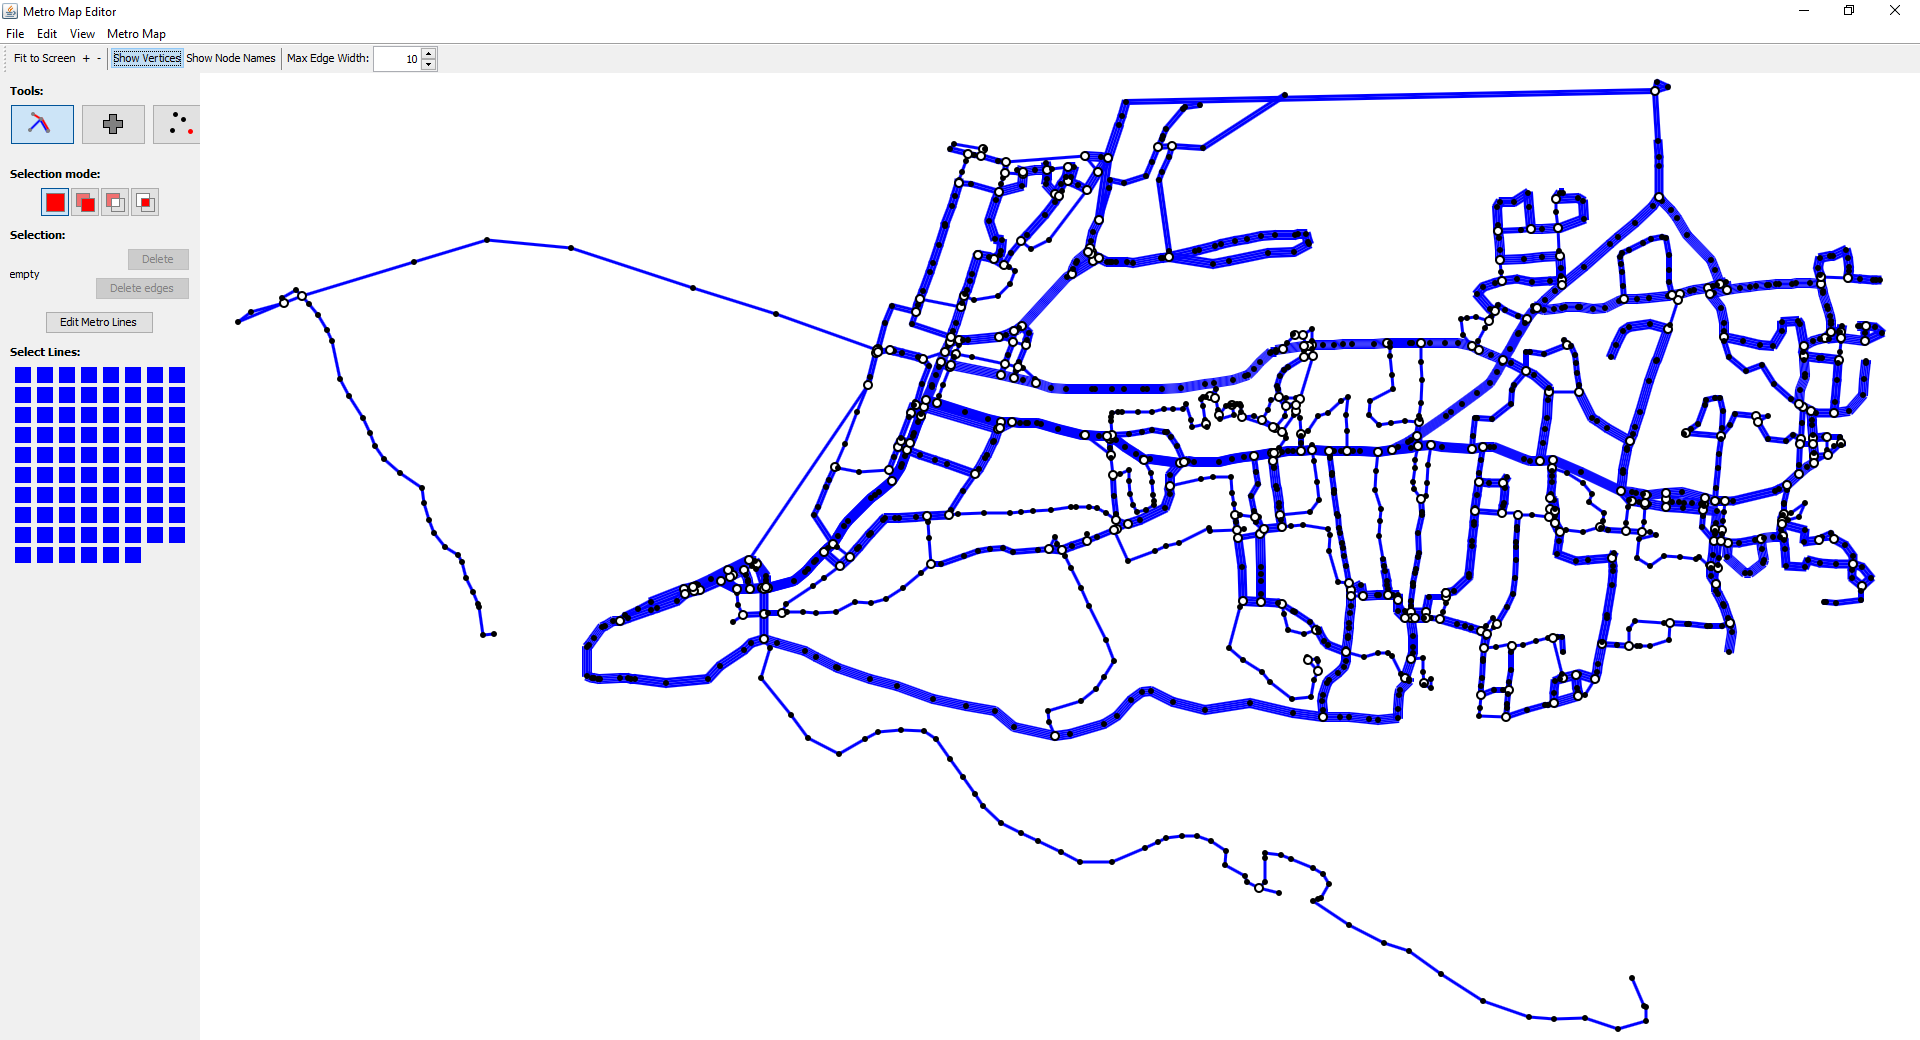
\includegraphics[height=0.35\textheight, trim=160 2 20 62, clip]{inicial_azul.png}\\
  {\scriptsize (a) Original}

  \vspace{0.15cm}
  \begin{columns}[c]
    \begin{column}{0.48\textwidth}
      \centering
      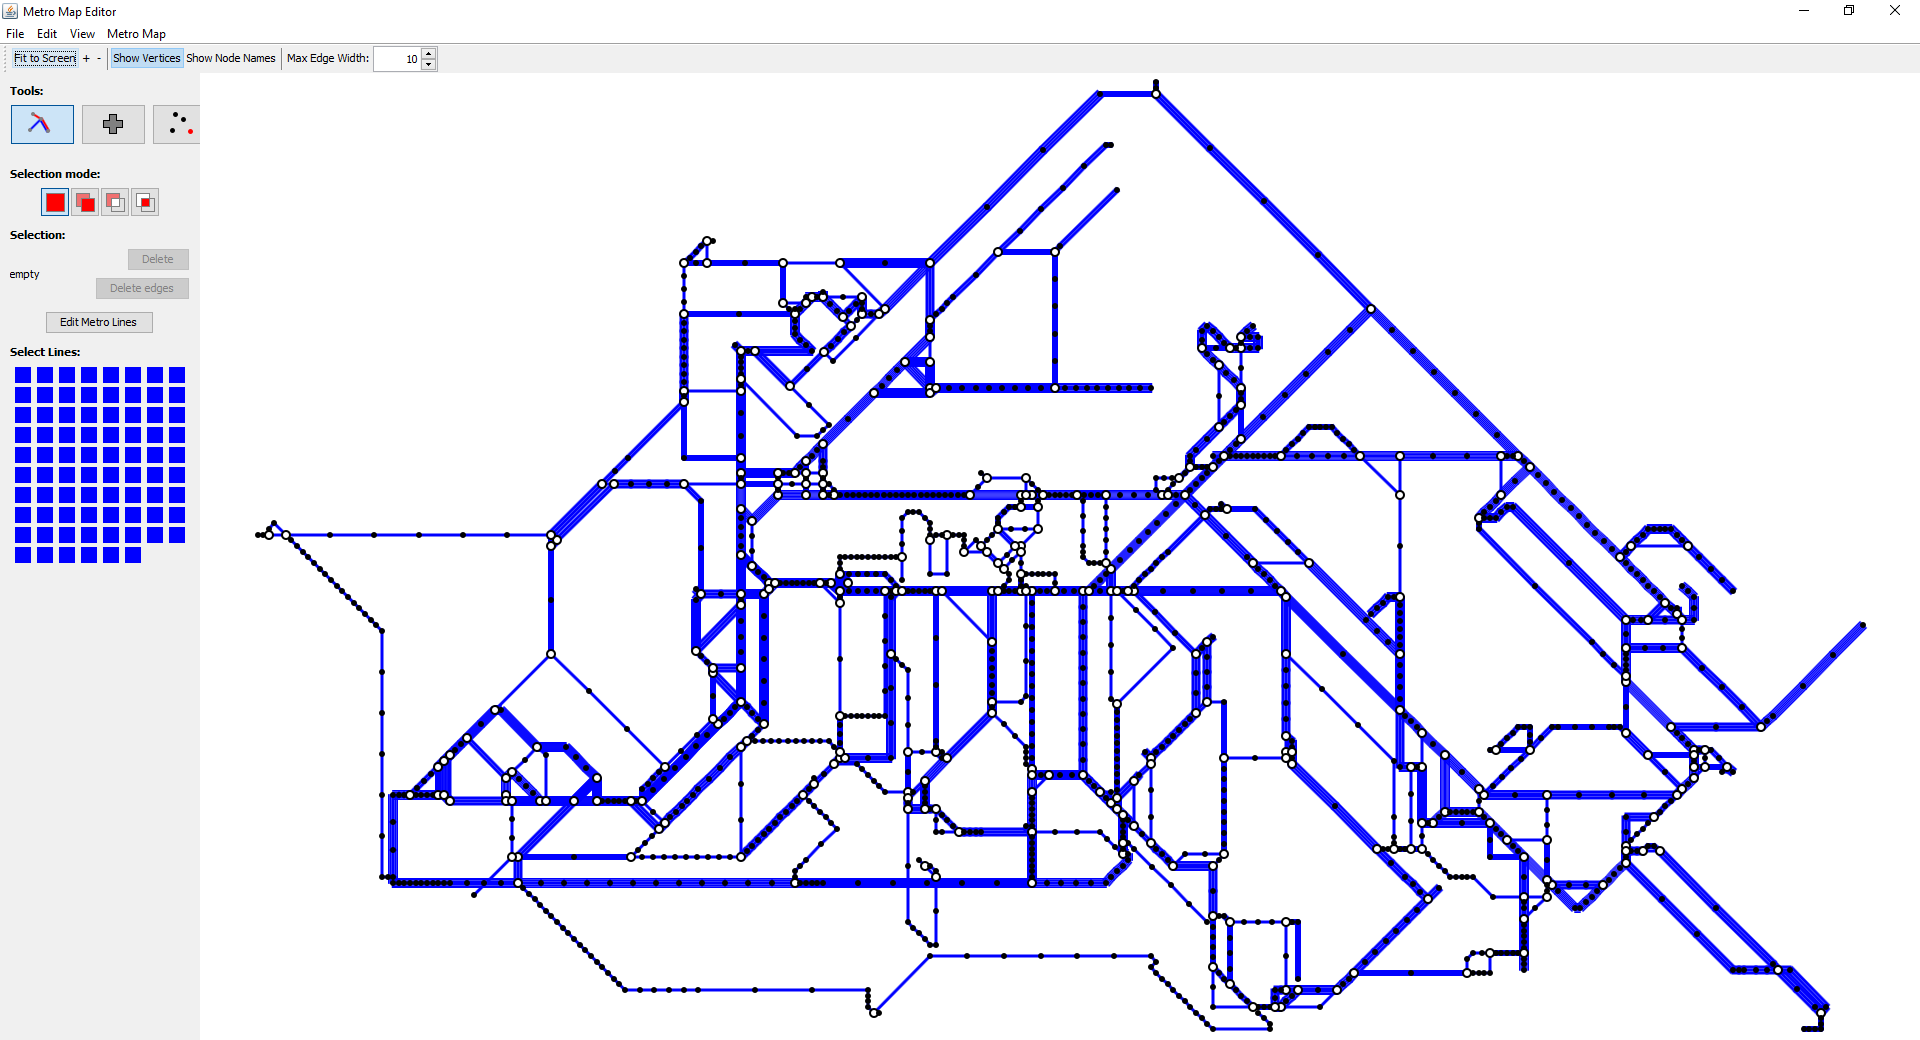
\includegraphics[height=0.35\textheight, trim=160 2 20 62, clip]{biobjetiva_azul.png}\\
      {\scriptsize (b) Biobjetivo (Gap 20\%)}
    \end{column}
    \begin{column}{0.48\textwidth}
      \centering
      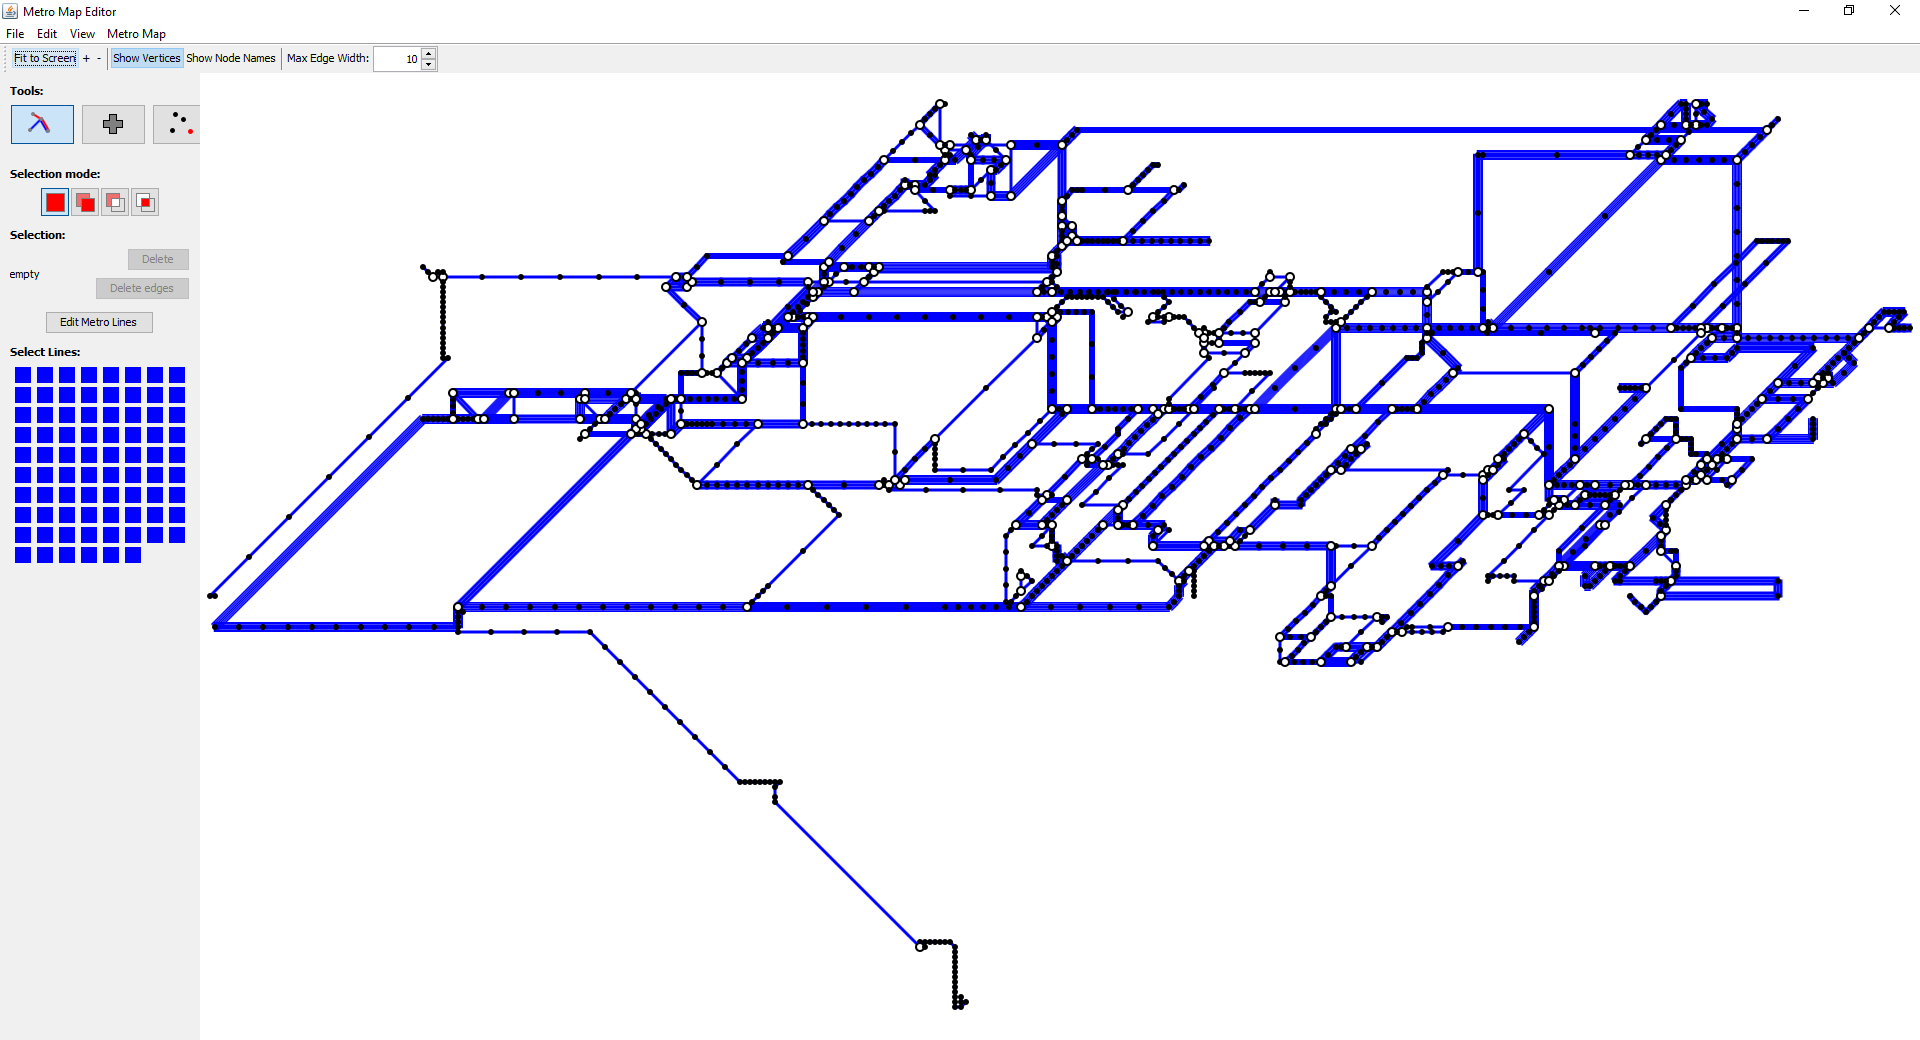
\includegraphics[height=0.35\textheight, trim=152 2 20 62, clip]{triobjetiva_azul.png}\\
      {\scriptsize (c) Triobjetivo (Gap 60\%)}
    \end{column}
  \end{columns}
\end{frame}

\begin{frame}{Resultado Qualitativo: Bacia Sul (Vermelha)}
  \centering
  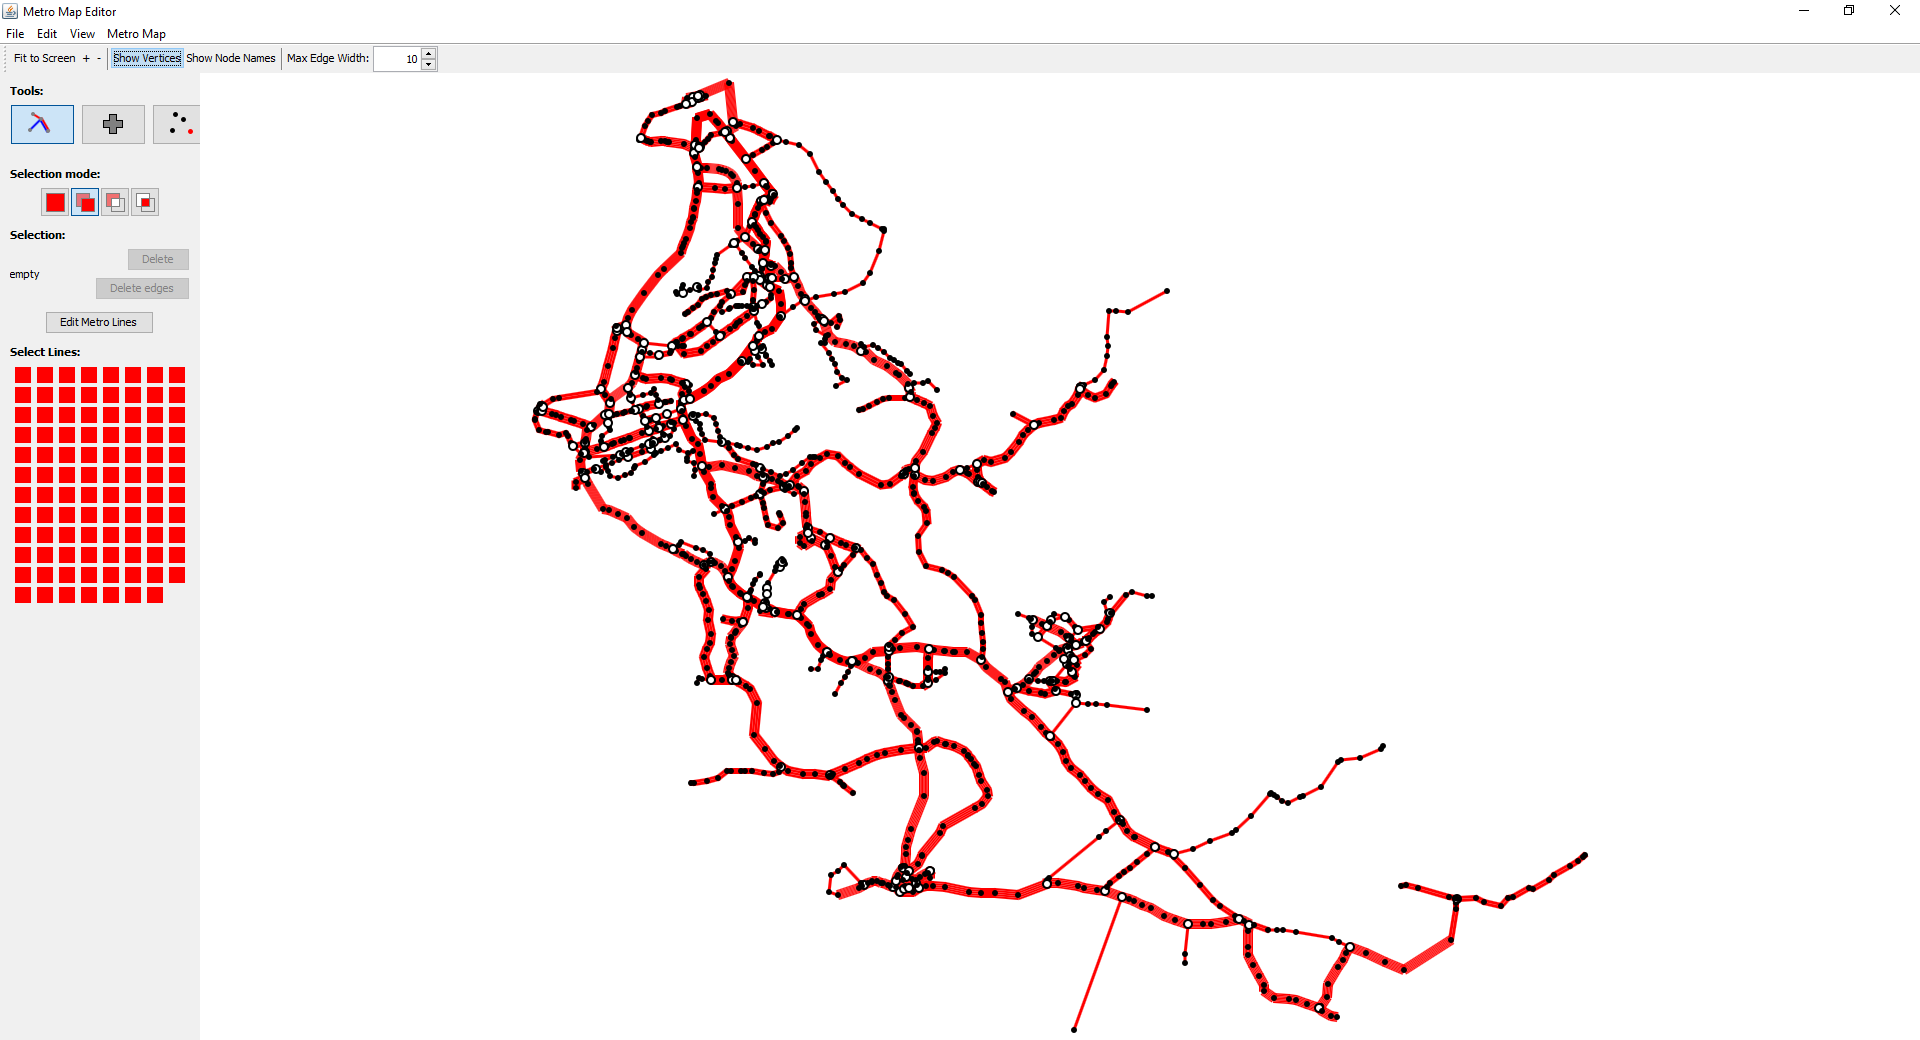
\includegraphics[height=0.35\textheight, trim=160 2 20 56, clip]{inicial_vermelho.png}\\
  {\scriptsize (a) Original}

  \vspace{0.15cm}
  \begin{columns}[c]
    \begin{column}{0.48\textwidth}
      \centering
      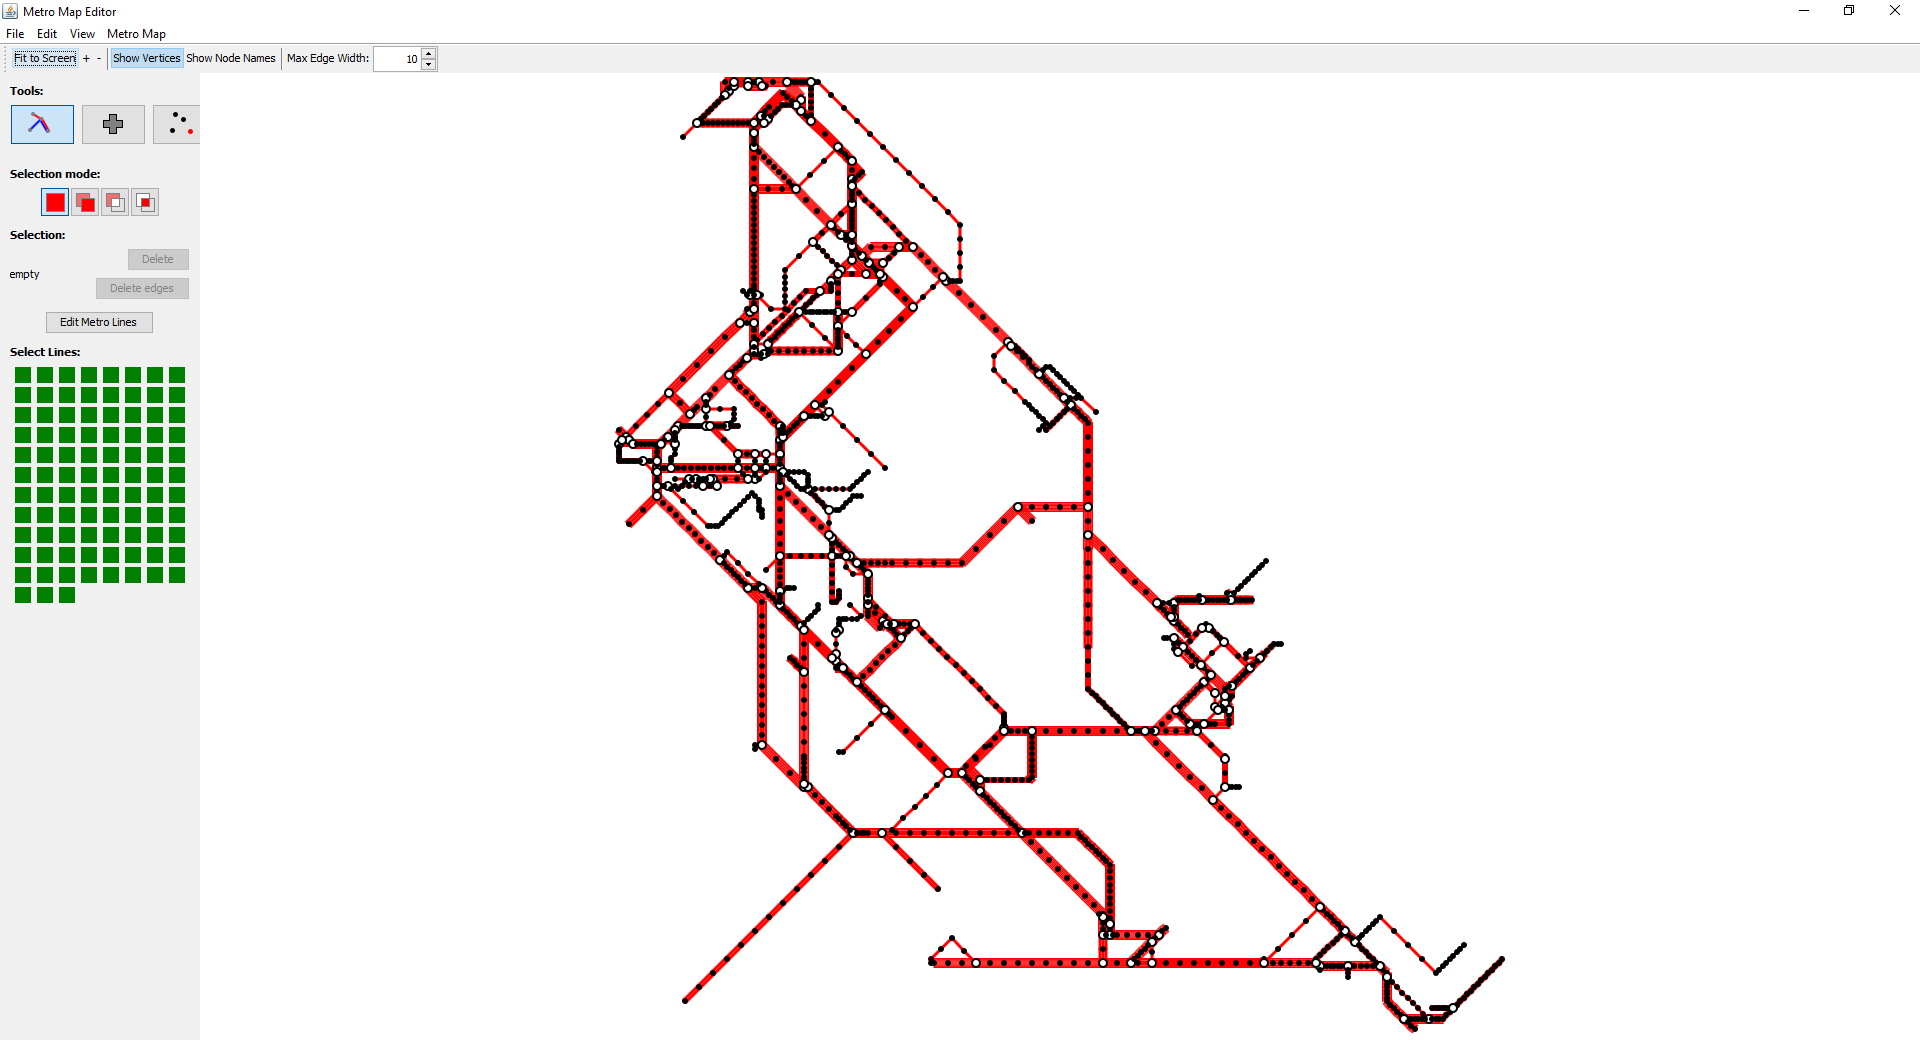
\includegraphics[height=0.35\textheight, trim=160 2 20 56, clip]{biobjetiva_vermelho.png}\\
      {\scriptsize (b) Biobjetivo (Gap 10\%)}
    \end{column}
    \begin{column}{0.48\textwidth}
      \centering
      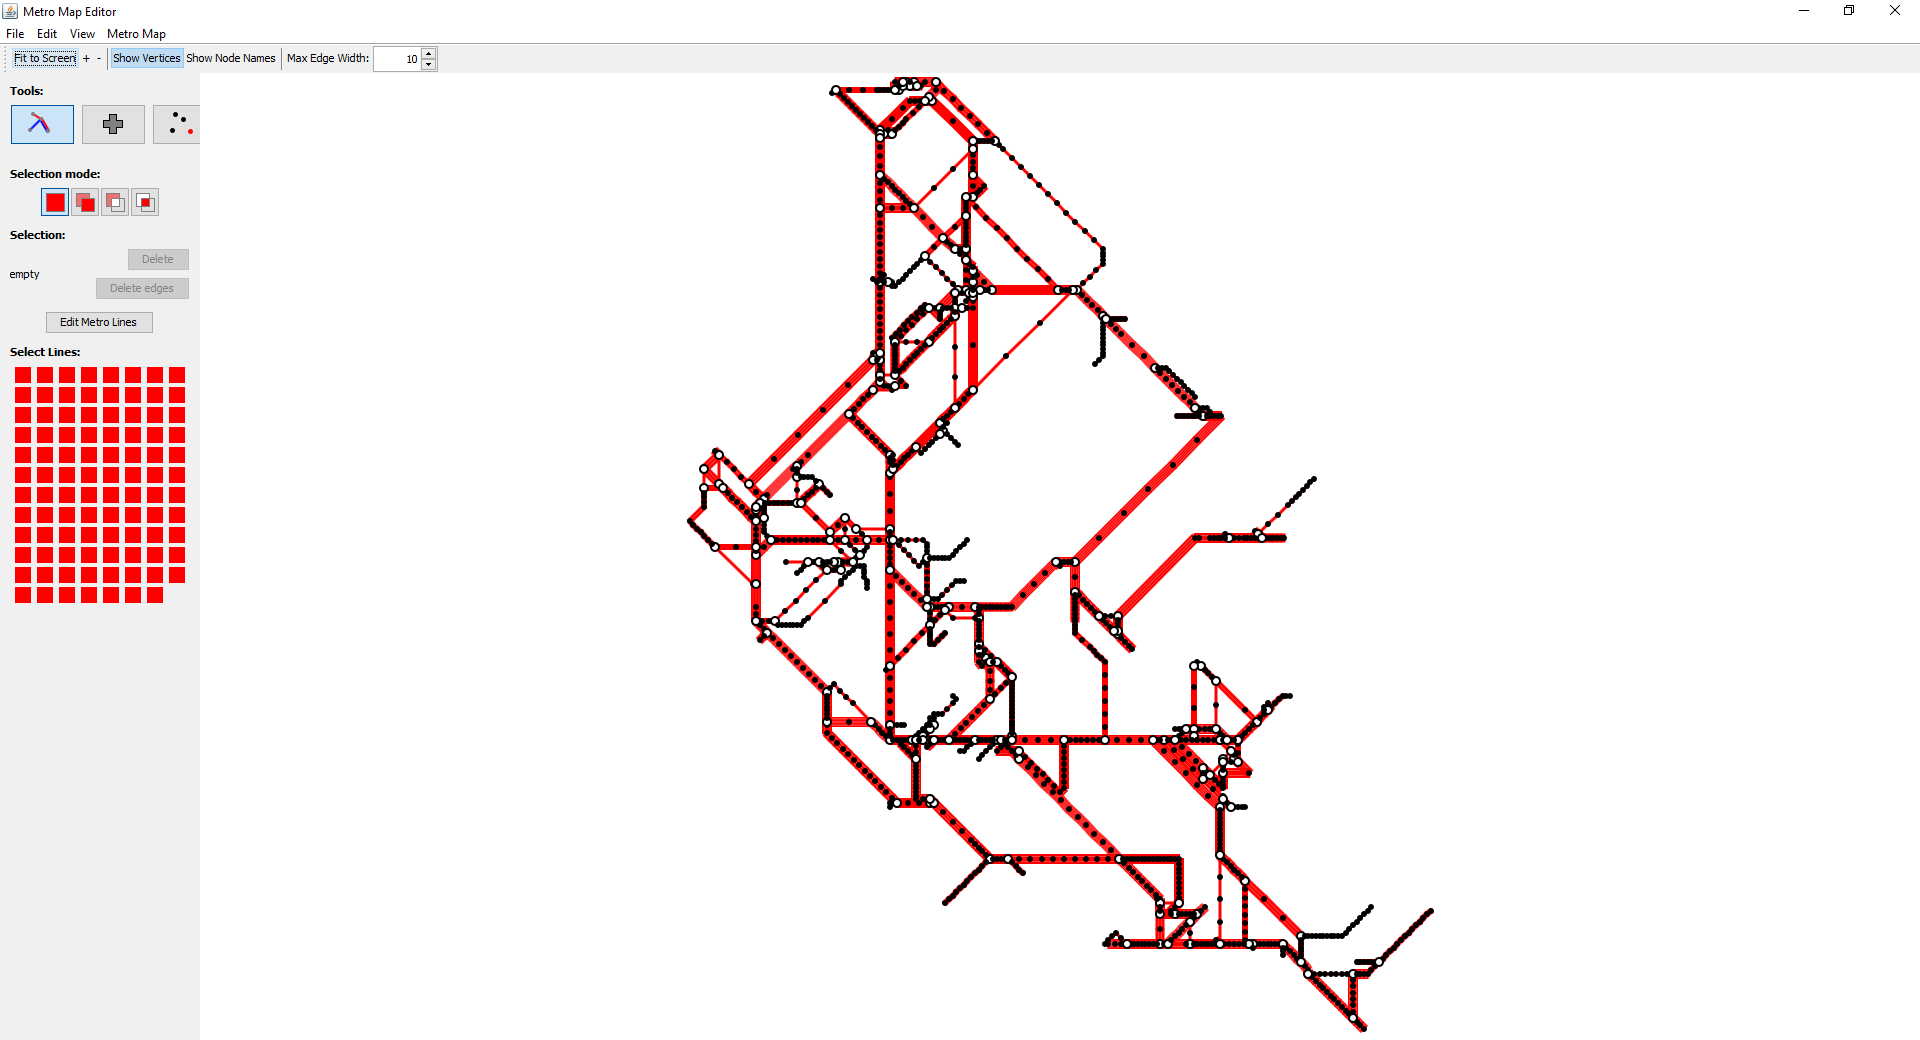
\includegraphics[height=0.35\textheight, trim=160 2 20 56, clip]{triobjetiva_vermelho.png}\\
      {\scriptsize (c) Triobjetivo (Gap 30\%)}
    \end{column}
  \end{columns}
\end{frame}

\begin{frame}{Resultado Qualitativo: Bacia Leste (Verde)}
  \centering
  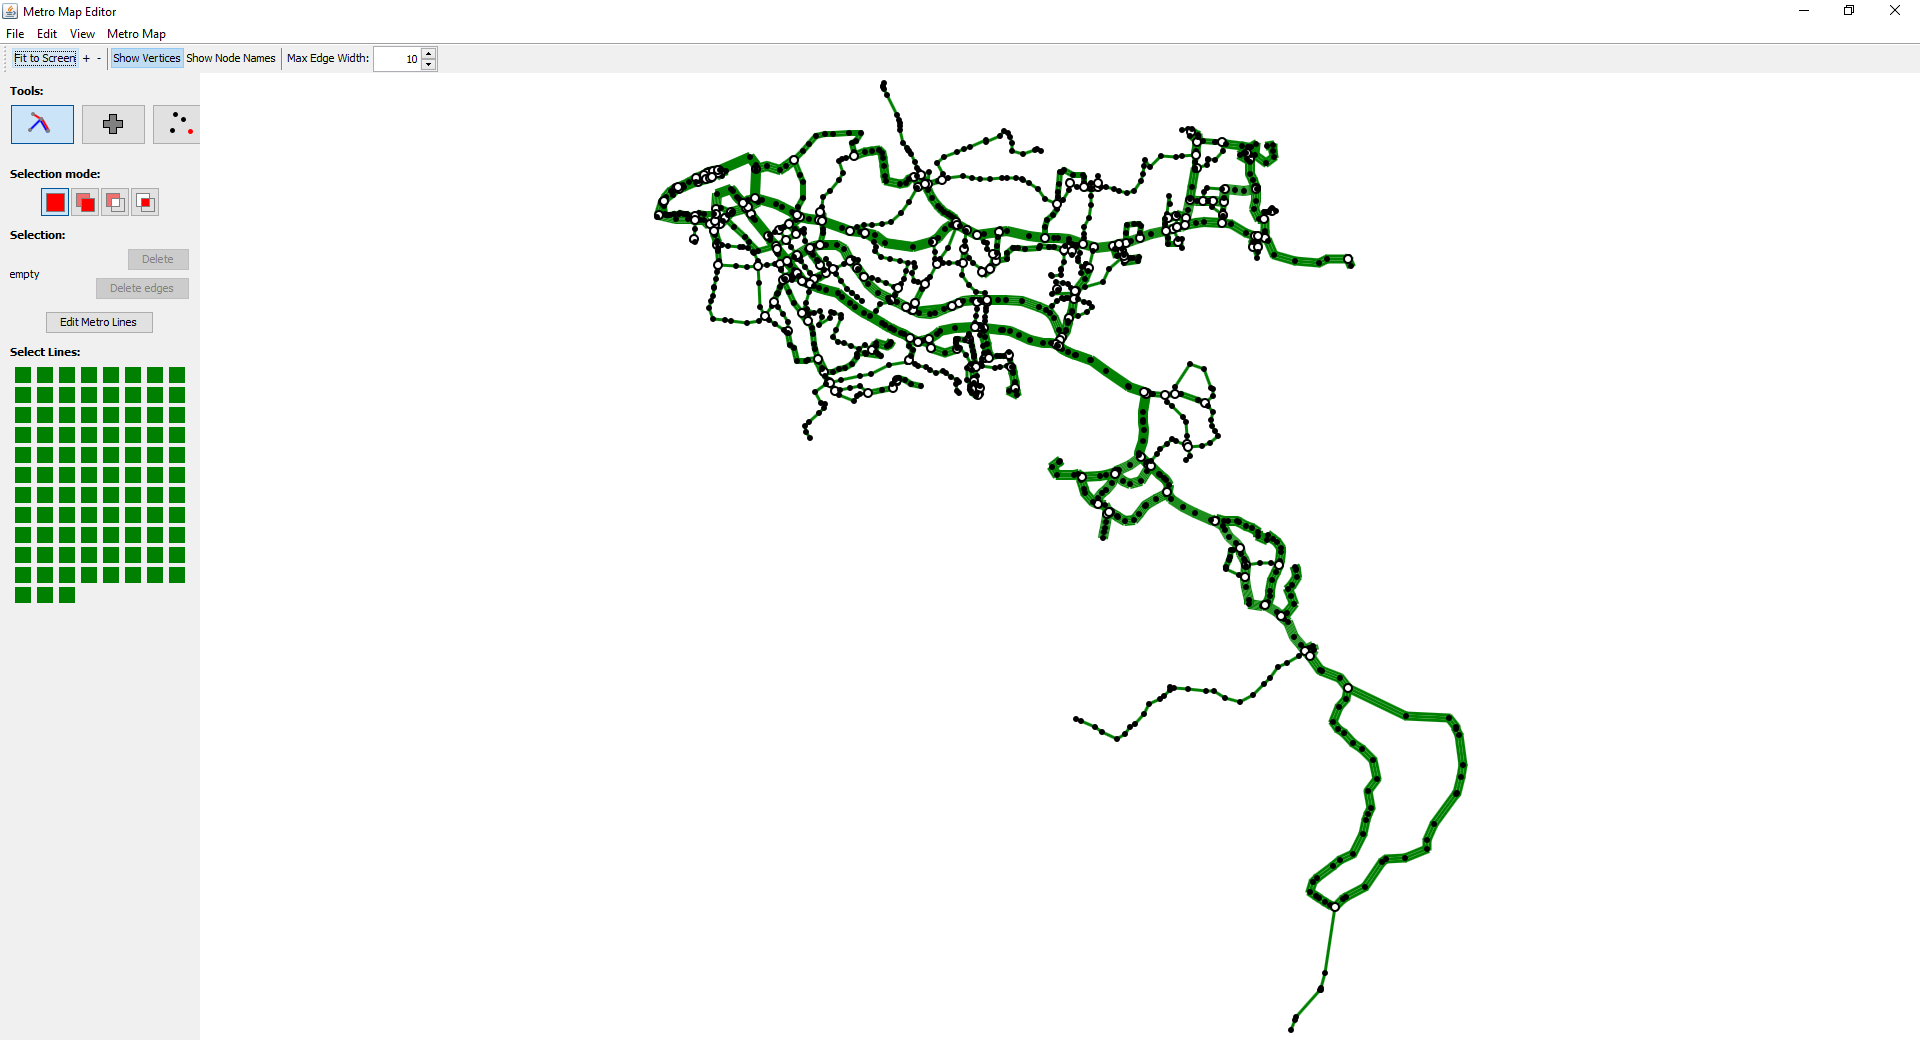
\includegraphics[height=0.35\textheight, trim=160 2 20 56, clip]{inicial_verde.png}\\
  {\scriptsize (a) Original}

  \vspace{0.15cm}
  \begin{columns}[c]
    \begin{column}{0.48\textwidth}
      \centering
      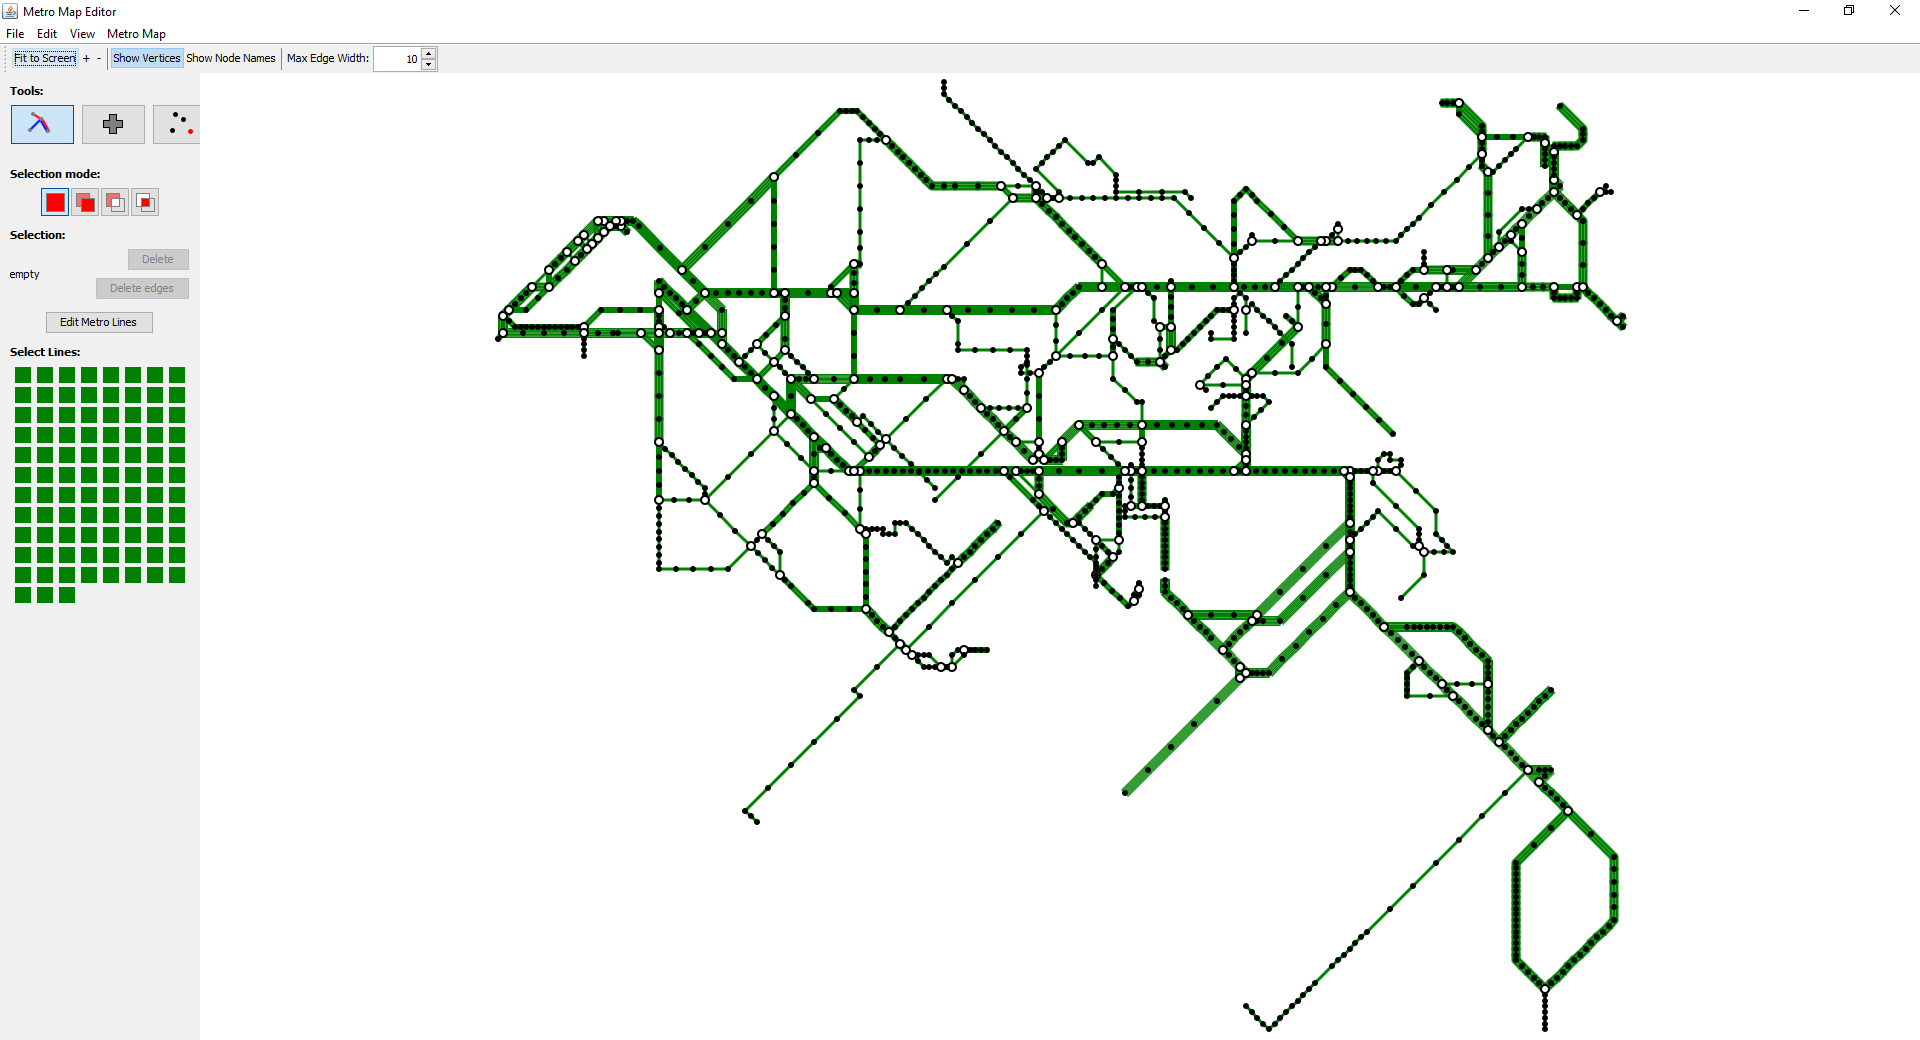
\includegraphics[height=0.35\textheight, trim=160 2 20 56, clip]{biobjetiva_verde.png}\\
      {\scriptsize (b) Biobjetivo (Gap 10\%)}
    \end{column}
    \begin{column}{0.48\textwidth}
      \centering
      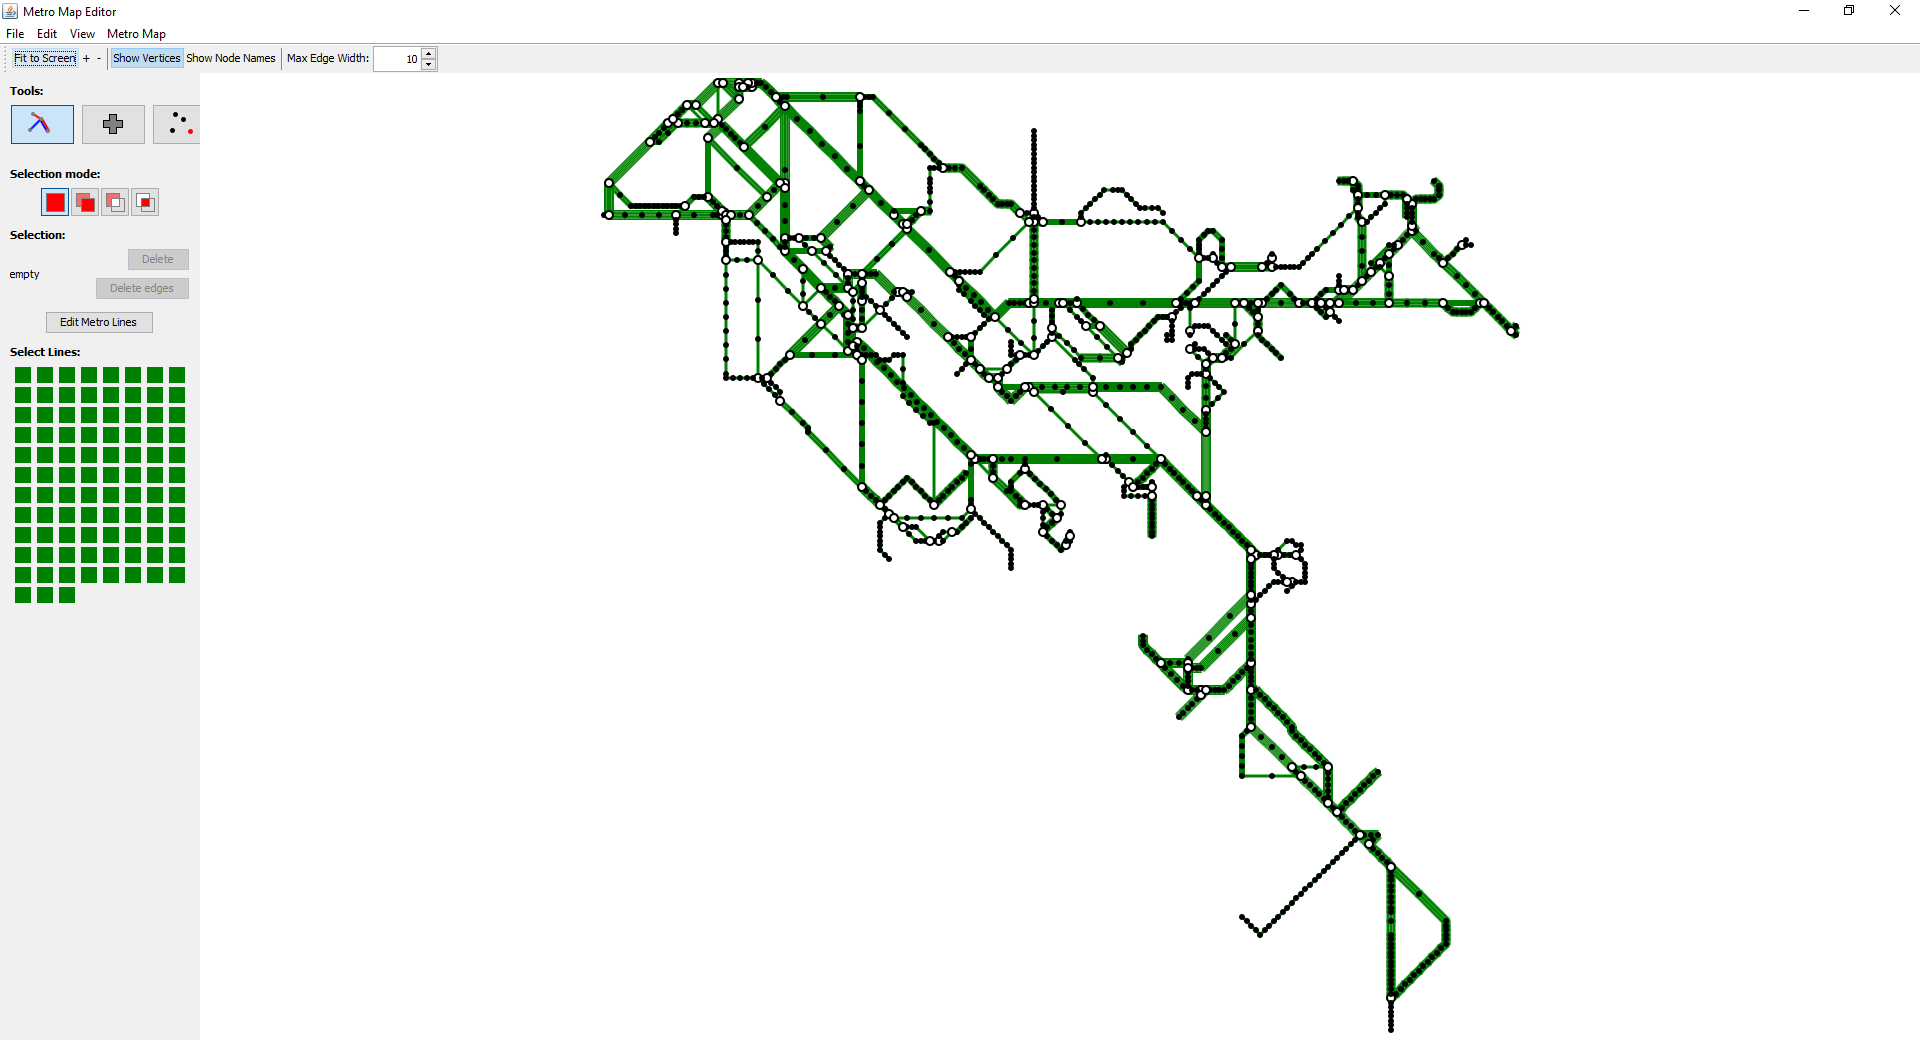
\includegraphics[height=0.35\textheight, trim=160 2 20 56, clip]{triobjetiva_verde.png}\\
      {\scriptsize (c) Triobjetivo (Gap 30\%)}
    \end{column}
  \end{columns}
\end{frame}

\begin{frame}{Resultado Qualitativo: Linhas Transversais (Laranja)}
  \centering
  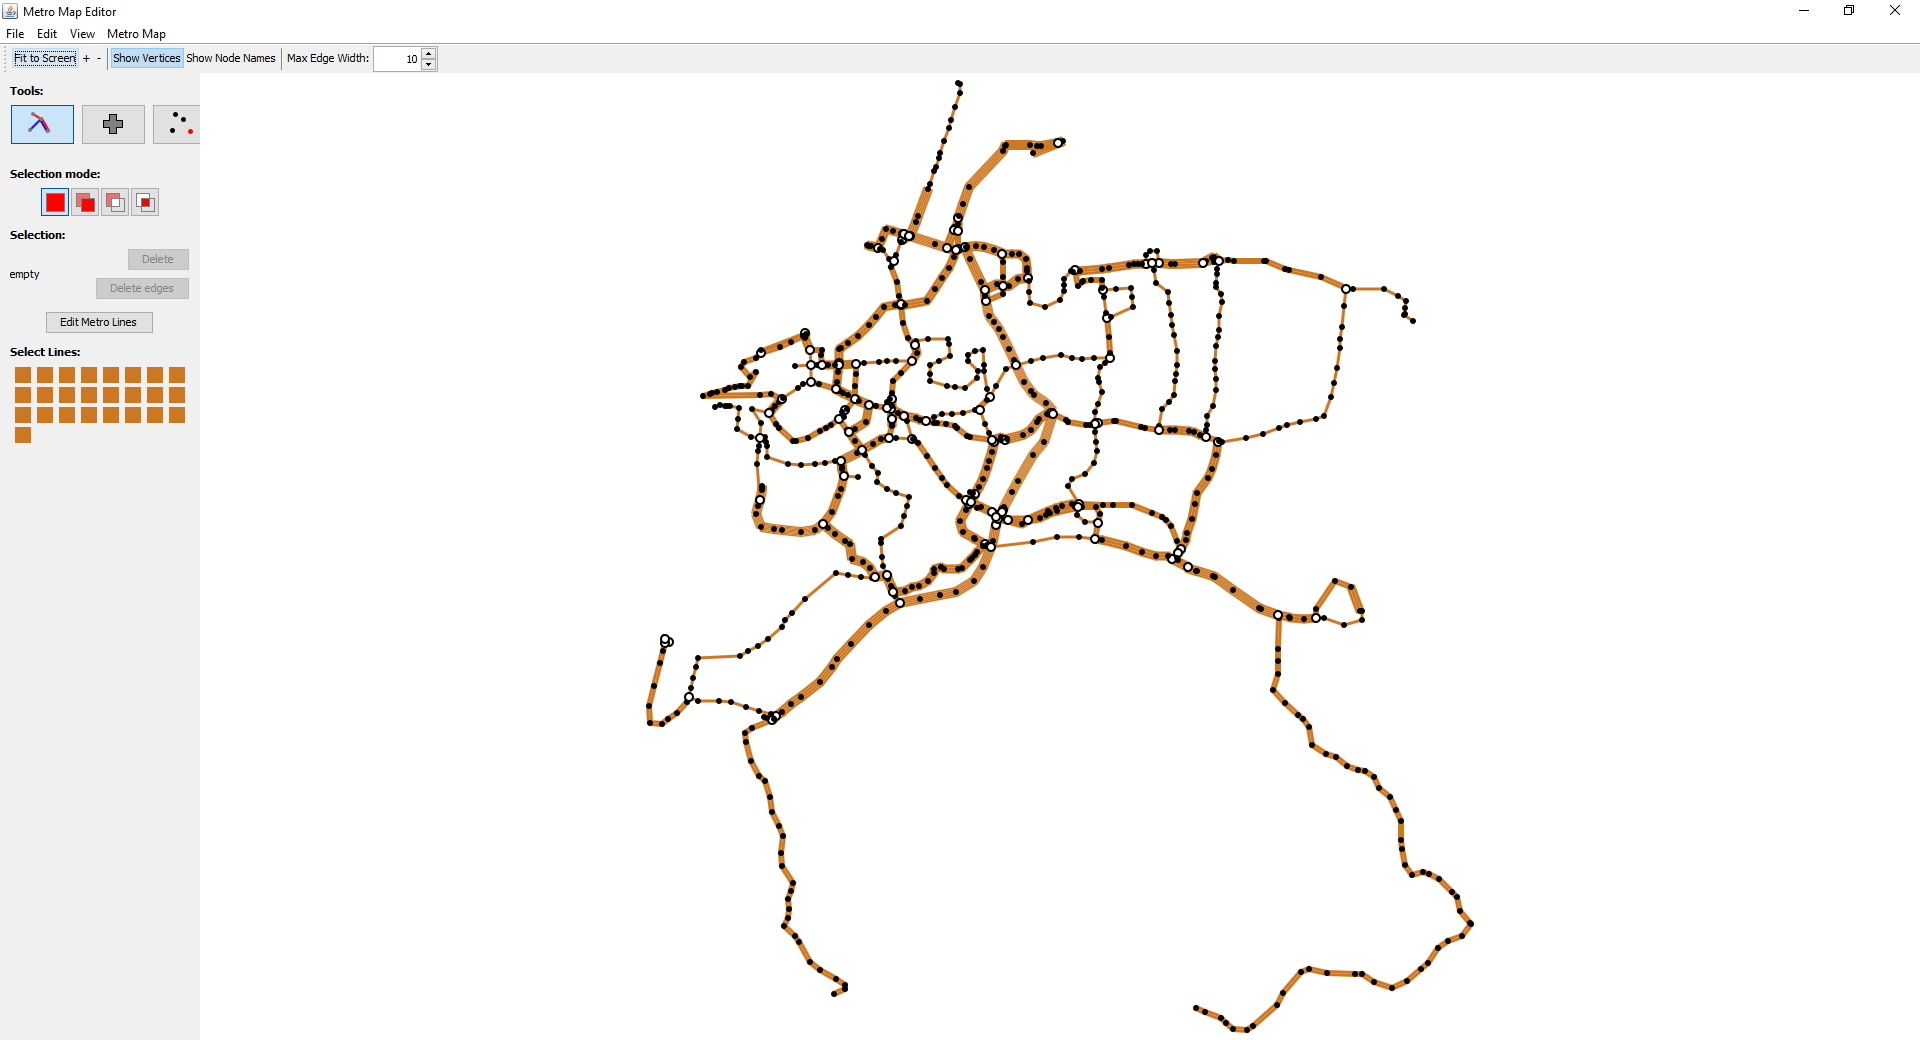
\includegraphics[height=0.35\textheight, trim=160 2 20 56, clip]{inicial_laranja.png}\\
  {\scriptsize (a) Original}

  \vspace{0.15cm}
  \begin{columns}[c]
    \begin{column}{0.48\textwidth}
      \centering
      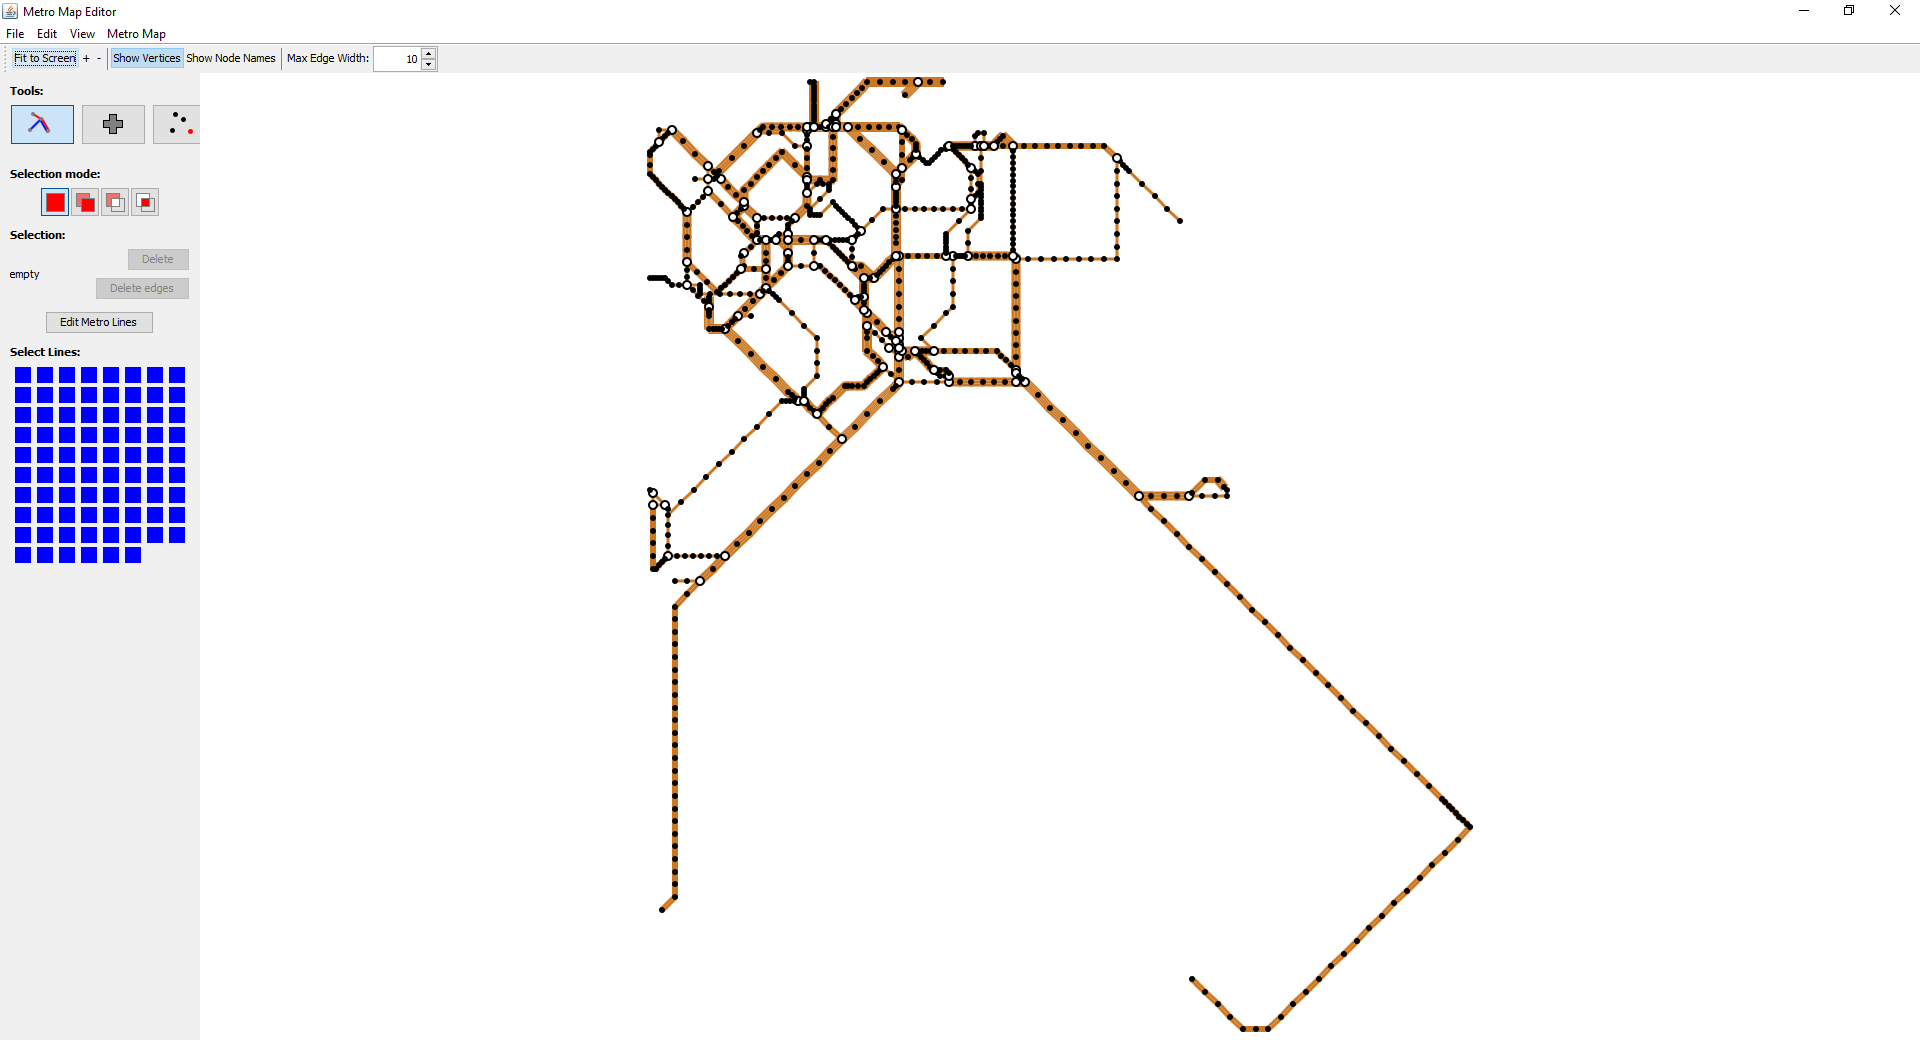
\includegraphics[height=0.35\textheight, trim=160 2 20 56, clip]{biobjetiva_laranja.png}\\
      {\scriptsize (b) Biobjetivo (Gap 10\%)}
    \end{column}
    \begin{column}{0.48\textwidth}
      \centering
      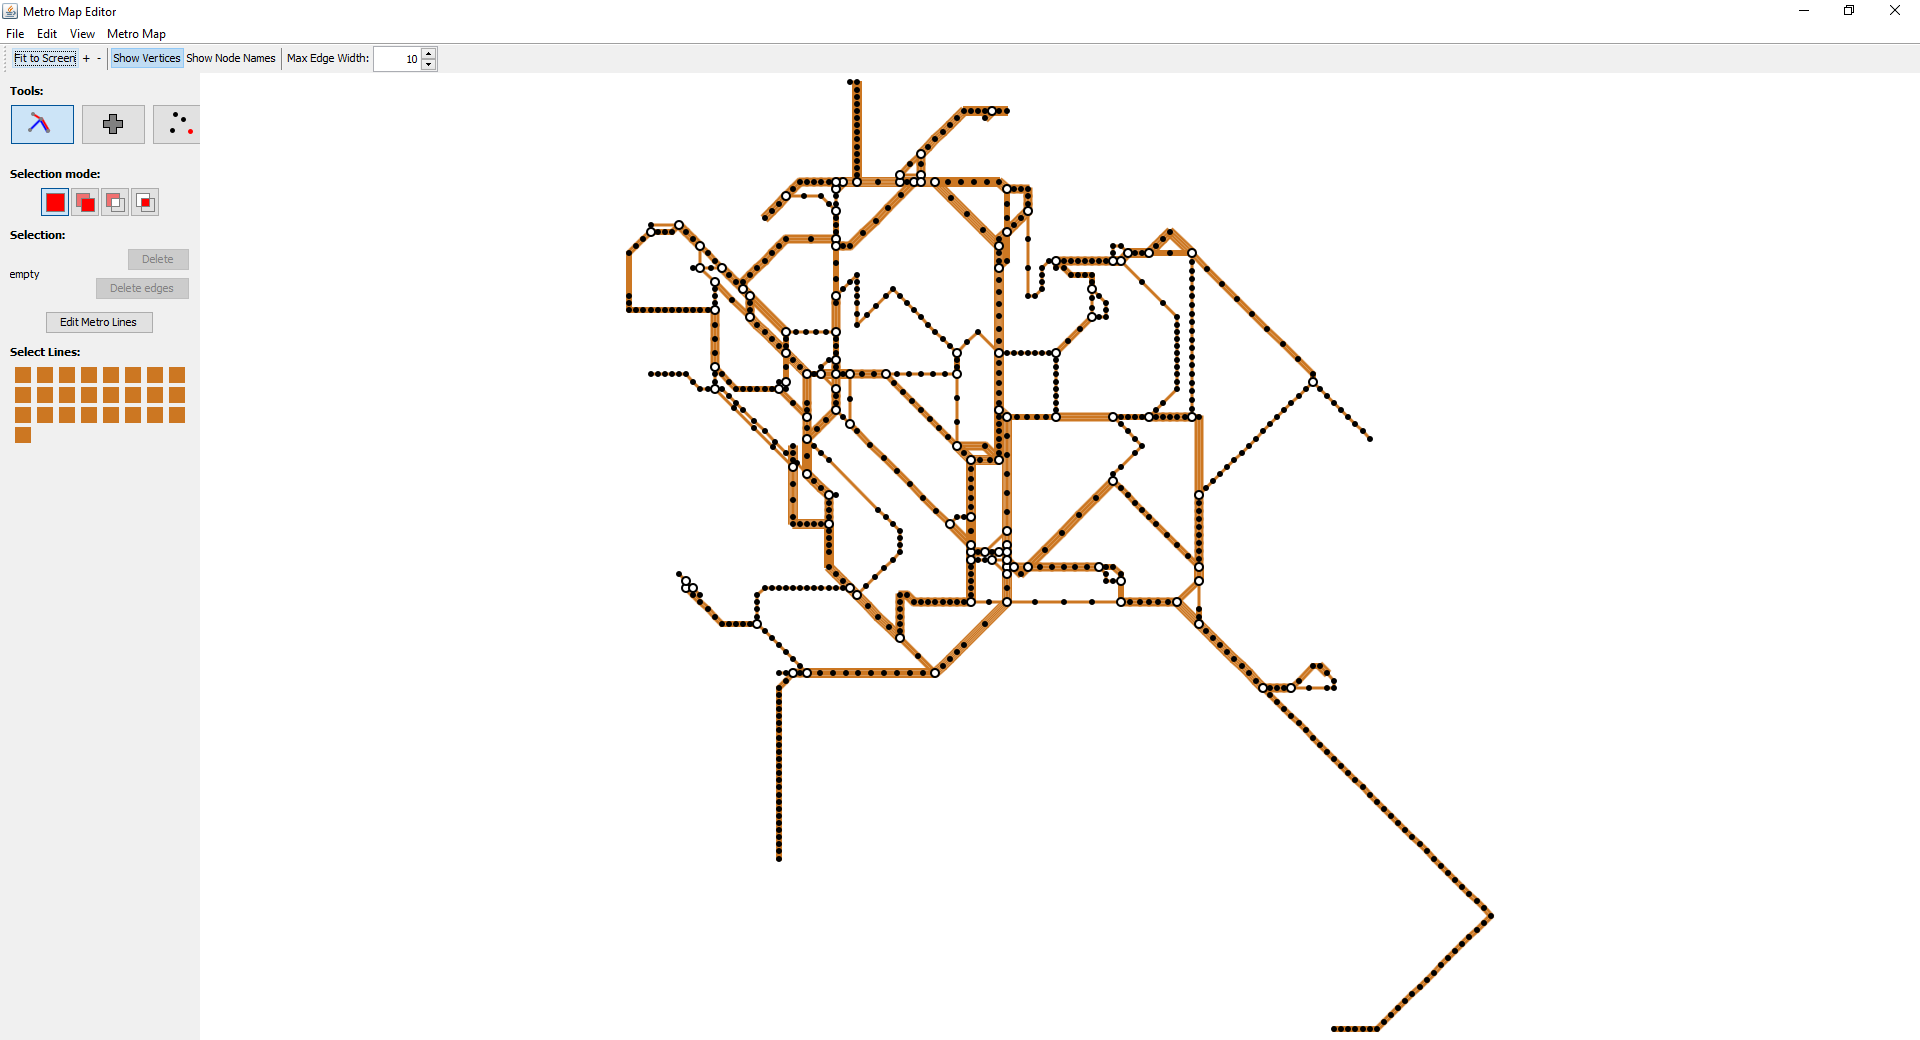
\includegraphics[height=0.35\textheight, trim=160 2 20 56, clip]{triobjetiva_laranja.png}\\
      {\scriptsize (c) Triobjetivo (Gap 20\%)}
    \end{column}
  \end{columns}
\end{frame}

\begin{frame}{Desempenho Computacional}
  \centering
  \resizebox{\textwidth}{!}{%
  \begin{tabular}{llrrrrr}
    \toprule
    \textbf{Bacia} & \textbf{Formulação} & \textbf{Iterações} & \textbf{Restr. Ang.} & \textbf{Tempo (s)} & \textbf{Cruz. Antes} & \textbf{Cruz. Depois} \\
    \midrule
    \multirow{2}{*}{Norte (Azul)}
      & Biobjetiva  & 44 & 2.435 & 33.394 & 85 & \textbf{4} \\
      & Triobjetiva & 50 & 3.638 & 18.841 & 22 & 12 \\
    \midrule
    \multirow{2}{*}{Sul (Vermelha)}
      & Biobjetiva  & 11 & 598   & \textbf{6.833}  & 32 & \textbf{4} \\
      & Triobjetiva & 34 & 462   & 31.496 & 9  & 10 \\
    \midrule
    \multirow{2}{*}{Leste (Verde)}
      & Biobjetiva  & 15 & 1.003 & \textbf{6.494}  & 49 & \textbf{5} \\
      & Triobjetiva & 14 & 476   & 10.491 & 23 & \textbf{5} \\
    \midrule
    \multirow{2}{*}{Transv. (Laranja)}
      & Biobjetiva  & 8  & 28    & \textbf{186}    & 3  & \textbf{0} \\
      & Triobjetiva & 3  & 31    & 415    & 1  & 1 \\
    \bottomrule
  \end{tabular}%
  }

  \vspace{0.2cm}
  {\small \textbf{Biobjetiva} $\rightarrow$ menos cruzamentos, menos tempo de execução, MIP Gap mais rigoroso.}
\end{frame}

% \begin{frame}{Biobjetiva vs.\ Triobjetiva — Síntese}
%   \begin{columns}[T]
%     \begin{column}{0.48\textwidth}
%       \textbf{Biobjetiva}
%       \begin{itemize}
%         \item Menor tempo de execução
%         \item MIP Gap mais rigoroso (10--20\%)
%         \item Até \textbf{3$\times$ menos cruzamentos}
%         \item Arestas regulares e homogêneas
%       \end{itemize}
%     \end{column}
%     \begin{column}{0.48\textwidth}
%       \textbf{Triobjetiva}
%       \begin{itemize}
%         \item Maior flexibilidade nas arestas
%         \item Melhor preservação de proporções em certas bacias
%         \item MIP Gap mais permissivo (20--60\%)
%         \item Custo computacional \textbf{substancialmente} maior
%       \end{itemize}
%     \end{column}
%   \end{columns}
% \end{frame}

% ============================================================
\section{Conclusão}
% ============================================================

\begin{frame}[plain]
  \sectionpage
\end{frame}

\begin{frame}{Conclusões}
  \begin{itemize}
    \item A esquematização via modelos de otimização linear é \textbf{factível e produz diagramas de qualidade} para bacias operacionais individuais em Porto Alegre através das etapas propostas:
    \begin{itemize}
      \item Pipeline de pré-processamento: \textbf{reduziu 58\% dos vértices} e o grau máximo de 8 para 5
      \item Pós-processamento iterativo: \textbf{corrigiu milhares de distorções} com custo computacional mínimo
      \item Formulação biobjetiva: melhor \textbf{qualidade e desempenho}
    \end{itemize}
    \item \alert{Barreira de escalabilidade:} rede completa permanece \textbf{intratável} para solvers MIP contemporâneos
  \end{itemize}
\end{frame}

\begin{frame}{Trabalhos Futuros}
  \begin{enumerate}
    \item \textbf{Aperfeiçoar o Grafo Híbrido:} aumentar taxa de retenção (92,89\% $\to$ 100\%)
    \item \textbf{Interface Gráfica (GUI) moderna:} camadas, filtros por bacia, zoom dinâmico
    \item \textbf{Posicionamento de rótulos:} algoritmos dedicados para redes densas
    \item \textbf{Calibração de parâmetros:} ângulos, grade, pesos
  \end{enumerate}
\end{frame}

% ============================================================
\section*{}
% ============================================================

\begin{frame}
  \frametitle{Obrigado!}

  \vspace{0.5cm}
  \centering
  {\Large\bfseries Perguntas?}

  \vspace{1cm}
  \begin{tabular}{rl}
    \textbf{Aluno:} & Gustavo Spellmeier Neves \\
    \textbf{Orientador:} & Prof.~Dr.~Lucas Melo Schnorr \\
    \textbf{Instituição:} & Instituto de Informática --- UFRGS \\
  \end{tabular}

  \vspace{0.8cm}
  \InfContacts
\end{frame}

\end{document}
